\documentclass[11pt]{article}
\usepackage[a4paper,margin=1in]{geometry}
\usepackage{amsmath,amssymb,amsthm,mathtools}
\usepackage[expansion=false]{microtype}
\usepackage{graphicx,booktabs,array}
\usepackage[font=small,labelfont=bf]{caption}
\usepackage[dvipsnames]{xcolor}
\usepackage{enumitem}
\usepackage[section]{placeins}
\usepackage[hidelinks,pdfusetitle]{hyperref}
\usepackage[nameinlink,capitalise]{cleveref}
\setlist{nosep,leftmargin=1.5em}
\newtheorem{theorem}{Theorem}[section]
\newtheorem{lemma}[theorem]{Lemma}
\newtheorem{proposition}[theorem]{Proposition}
\newtheorem{corollary}[theorem]{Corollary}
\theoremstyle{definition}\newtheorem{definition}[theorem]{Definition}
\theoremstyle{remark}\newtheorem{remark}[theorem]{Remark}
\theoremstyle{definition}\newtheorem{axiom}{Axiom}
\newcommand{\R}{\mathbb R}\newcommand{\C}{\mathbb C}\newcommand{\N}{\mathbb N}\newcommand{\Z}{\mathbb Z}
\newcommand{\dd}{\,\mathrm d}\newcommand{\e}{\mathrm e}
\renewcommand{\Re}{\operatorname{Re}}\renewcommand{\Im}{\operatorname{Im}}
\newcommand{\fr}[1]{\{#1\}}
\newcommand{\li}{\operatorname{li}}\newcommand{\Tr}{\operatorname{Tr}}
\setlength{\parskip}{0.35em}
\AtBeginDocument{\sloppy}
\urlstyle{same}
\hypersetup{pdftitle={The Square-Root Horizon: Squares, Reversal and Prime Clocks},pdfauthor={Abhijit Singh}}
\title{\textbf{The Square-Root Horizon:}\\[4pt]
\large Squares, Reversal and Prime Clocks in the Distribution of the Primes\\ and the Zeros of the Riemann Zeta Function}
\author{Abhijit Singh}
\date{}
\begin{document}
\maketitle
\begin{abstract}
We read the primes and the zeros of the Riemann zeta function through three exact structures: the residue classes of the divisor $r$ in the rebuild law $\sum_{r\le x}M(x/r)=1$ for the Mertens function, the squares of the primes, and the reversal of the Euler product. Split by $r\bmod3$ the rebuild law is $(1,a(x),-a(x))$ for $x\ge3$, with $a(x)=\frac12\sum_{k\le x}(\mu*\chi_{-3})(k)$ carried only by $3$ and the primes $\equiv2\pmod3$; split by $r\bmod4$ it is $(1,b(x),0,-b(x))$. The zero class reproduces the whole law at $x/3$, so the classes modulo $3^\kappa$ form a self-similar tower with an exact energy recursion whose leaves are the values $M(x/r)$; the leaf energy is $\ll x^{1+\varepsilon}$ for every $\varepsilon>0$ if and only if the Riemann Hypothesis (RH) holds. At every zero $\rho$ of $\zeta$ the three classes of the Dirichlet series stand as $(0,\frac12L(\rho,\chi_{-3}),-\frac12L(\rho,\chi_{-3}))$. An exact sieve to $10^{10}$ in integer and Eisenstein-integer arithmetic gives every class value at $10^{10}$, and the wave amplitudes of $a(x)/\sqrt x$ at the first twelve zeros agree with $|L(\rho,\chi_{-3})/\rho\zeta'(\rho)|$ to within $0.0003$, including a sixth wave of amplitude $0.0012$ against $0.0011$ predicted. For consecutive primes $p<p'$ the primes in $[p,pp')$ together with $p^2$ are exactly the integers there free of the primes below $p$; with $25$ and $49$ inserted, the gaps from $5$ to $59$ are $2,4,2,4,2,4,2,4,2,6,4,2,4,2,4,6$ and the classes $6k\pm1$ up to $61$ stand $9:9$. Each prime square enters the logarithm of the Euler product with weight $\frac12$, and at that weight the lean of the prime count vanishes: over $2^{12}\le x\le10^{10}$ the mean of $(\pi(x)-\li(x))\log x/\sqrt x$ is $-1.364$, that of $(J(x)-\li(x)+\log2)\log x/\sqrt x$ is $+0.0013$, and the square weight that balances the count, fitted from the data, is $0.4994$; the lean of the Liouville sum is carried by its square multiples, $L(x)-M(x)=\sum_{d\ge2}M(x/d^2)$, and that of the classes $6k\pm1$ by the prime squares, which all lie in the class $6k+1$ and at weight $\frac12$ reduce it from $1.157$ to $0.031$ in units of $\sqrt x/\log x$. The squares part $E(s)=\exp\sum_p\sum_{k\ge2}p^{-ks}/k$ of $\zeta$ is analytic and zero-free for $\sigma>\frac12$, satisfies $E(\sigma)^3|E(\sigma+it)|^4|E(\sigma+2it)|\ge1$ there, and has at $s=\frac12$ a half-order pole matched by a half-order zero of the prime factor $\zeta/E$, which carries every zero of $\zeta$ in $\sigma>\frac12$. In the model with independent uniform phases, the joint limit law of the phases $t\log p$, which unique factorisation makes linearly independent over the rationals, the random prime sum converges almost surely exactly for $\sigma>\frac12$ and its variance is the squares series $\sum_pp^{-2\sigma}$; at heights $5000$ to $6000$ the distribution of $\log|\zeta(\sigma+it)|$ for $\sigma=0.6,0.7,0.8$ follows this law, with standard deviations within $2.5\%$. Reversing the sign of every prime turns $\zeta(s)$ into $\zeta(2s)/\zeta(s)$, the zeros of $\zeta$ into poles and the product of the two patterns into $\zeta(2s)$; we prove $\sum_{n\le x}L(x/n)=\lfloor\sqrt x\rfloor$ and $-\sum_{k\ge1}\lambda(k)\fr{x/k}=\lfloor\sqrt x\rfloor$ for every $x>0$, and that if the sawtooths $\fr{1/(kt)}$ approximate the odd-square staircase $[\lfloor t^{-1/2}\rfloor\text{ odd}]$ in $L^2(0,\infty)$ then every zero of $\zeta$ in the critical strip lies on the line $\sigma=\frac12$. Computed from exact integrals for up to $2000$ sawtooths, the mean of $D_N^2\log N$ over $1200\le N\le2000$ lies $2.5\%$ above $\sum_\rho|\eta(2\rho)|^2/|\rho|^2=0.0750$, beside $0.6\%$ below $2+\gamma_E-\log4\pi=0.0462$ for $d_N^2\log N$ with the unit step. The Dirichlet series $\eta(2s)/\zeta(s)$ of the exact weights of the staircase vanishes at $s=1$. Cut at $N$, these weights therefore settle the part of the distance over $t>1$. Over $0<t\le1$ they leave an error of $0.058$ to $0.281$ for $300\le N\le2000$, so $D_N\to0$ rests on coefficients chosen afresh at each $N$. At every zero, the zero of the forward pattern and the pole of the reversed pattern cancel in their product, with residue $\zeta(2\rho)/\zeta'(\rho)$, in the same way on the line and off it. Over the $2469$ zeros below height $3000$ Landau's formula holds to within $0.0038$ at all $35$ prime powers up to $100$: each prime pulls the zeros toward the reversal $p^{i\gamma}=-1$ of its clock, the zeros are $0.65$ to $0.68$ times as dense near the alignment $2^{i\gamma}=1$ as on average, and the tenth zero, at $5.4909$ turns of the clock of $2$, is silenced in the reversed reading by the factor $1-2^{1-2s}$. In this language RH is the statement that every pole of the reversed pattern lies on the vertical line through its centre $s=\frac12$. We state the axiom of harmonic independence: the prime waves, whose frequencies $\log p$ are linearly independent by unique factorisation, are related only through the mechanism of their construction, and a zero off the critical line would be a relation without a mechanism.
\end{abstract}

\tableofcontents

\section{Introduction}\label{sec:intro}

Let $\mu$ be the Möbius function, $\lambda$ the Liouville function and $\Lambda$ the von Mangoldt function, and let $M(x)=\sum_{n\le x}\mu(n)$, $L(x)=\sum_{n\le x}\lambda(n)$, $\pi(x)$, $\theta(x)=\sum_{p\le x}\log p$, $\psi(x)=\sum_{n\le x}\Lambda(n)$ and $J(x)=\sum_{k\ge1}\pi(x^{1/k})/k$; functions of $x$ vanish for $x<1$. We write $\pi(x;q,a)$, $\theta(x;q,a)$ and $\psi(x;q,a)$ for the same counts restricted to $n\equiv a\pmod q$, $\li(x)$ for the logarithmic integral, $\chi_{-3}$ and $\chi_{-4}$ for the nonprincipal characters modulo $3$ and $4$, $L(s,\chi)$ for Dirichlet $L$-functions, $\zeta(s,a)$ for the Hurwitz zeta function and $\eta(s)=\sum_{n\ge1}(-1)^{n-1}n^{-s}=(1-2^{1-s})\zeta(s)$; $\nu(n)$ and $\Omega(n)$ are the numbers of distinct and of all prime factors of $n$, and $\gamma_E$ is Euler's constant. The nontrivial zeros of $\zeta$ are $\rho=\beta+i\gamma$, counted with multiplicity; $N(T)$ is the number with $0<\gamma\le T$. The Riemann Hypothesis (RH) is the statement that $\beta=\frac12$ for every $\rho$. All zeros with $0<\gamma\le3\cdot10^{12}$ lie on the line $\sigma=\frac12$ \cite{PT}. We measure $x$ in doublings, $u=\log_2x$; a zero $\frac12+i\gamma$ contributes to the counts a wave $x^{i\gamma}=\e^{2\pi i\,u\,\gamma\log2/2\pi}$ whose pitch is $\gamma\log2/2\pi$ turns per doubling.

In \cite{S10} the pairing of the squarefree divisors $\{d,dp\}$ of every integer $k>1$ gave the rebuild law
\begin{equation}\label{eq:rebuild}
\sum_{r\le x}M(x/r)=1\qquad(x\ge1),
\end{equation}
by which the balance of the Möbius sum at every scale is fixed by the balances at all smaller scales. The present paper reads the law, the prime counts and $\zeta$ itself through three exact structures: the residue classes of the divisor $r$ in \eqref{eq:rebuild}; the squares of the primes, which sit on the square-root horizon $\sigma=\frac12$ where the series $\sum_pp^{-2\sigma}$ stops converging; and the reversal $p\mapsto-p$ of the Euler product, which turns every zero of $\zeta$ into a pole.

\subsection{Main results}

For $m\ge1$, a residue $c\bmod m$ and a character $\chi\bmod m$ put
\begin{equation}\label{eq:classsum}
S^{(m)}_c(x)=\sum_{\substack{r\le x\\ r\equiv c\ (m)}}M(x/r),\qquad G_\chi(x)=\sum_{r\le x}\chi(r)M(x/r)=\sum_{k\le x}(\mu*\chi)(k),
\end{equation}
and write $G_{-3}=G_{\chi_{-3}}$, $G_{-4}=G_{\chi_{-4}}$.

\begin{theorem}[the triad tower]\label{mt:tower}
\begin{enumerate}[label=\textup{(\roman*)}]
\item For $x\ge3$, $\bigl(S^{(3)}_0,S^{(3)}_1,S^{(3)}_2\bigr)(x)=\bigl(1,a(x),-a(x)\bigr)$ with $a(x)=\frac12G_{-3}(x)$; for $x\ge4$, $\bigl(S^{(4)}_0,S^{(4)}_1,S^{(4)}_2,S^{(4)}_3\bigr)(x)=\bigl(1,b(x),0,-b(x)\bigr)$ with $b(x)=\frac12G_{-4}(x)$.
\item For $\kappa\ge0$, every $c$ and every $x>0$, $S^{(3^{\kappa+1})}_{3c}(x)=S^{(3^\kappa)}_c(x/3)$; for a unit $v\bmod3^\kappa$, $S^{(3^\kappa)}_v(x)=\varphi(3^\kappa)^{-1}\sum_{\chi\bmod3^\kappa}\overline\chi(v)G_\chi(x)$.
\item The energy $\mathcal E_\kappa(x)=\sum_{c\bmod3^\kappa}S^{(3^\kappa)}_c(x)^2$ of level $\kappa$ satisfies
\begin{equation}\label{eq:energyrec}
\mathcal E_\kappa(x)=\mathcal E_{\kappa-1}(x/3)+\frac1{\varphi(3^\kappa)}\sum_{\chi\bmod3^\kappa}|G_\chi(x)|^2\qquad(\kappa\ge1).
\end{equation}
\item If $3^\kappa>x$ the classes are the leaves $S^{(3^\kappa)}_r(x)=M(x/r)$, and $\mathcal E_\infty(x)=\sum_{r\le x}M(x/r)^2$. RH holds if and only if $\mathcal E_\infty(x)\ll_\varepsilon x^{1+\varepsilon}$ for every $\varepsilon>0$.
\end{enumerate}
\end{theorem}

\begin{theorem}[the carriers]\label{mt:carriers}
For every character $\chi$, prime $p$ and $e\ge1$, $(\mu*\chi)(p^e)=\chi(p)^{e-1}(\chi(p)-1)$. Hence $\mu*\chi$ vanishes on every multiple of a prime $p$ with $\chi(p)=1$; for $\chi\bmod m$ this includes every prime $p\equiv1\pmod m$. In particular $\mu*\chi_{-3}$ is supported on the integers $3^jn$ with $j\in\{0,1\}$ and $n$ composed of primes $\equiv2\pmod3$, where $(\mu*\chi_{-3})(3^jn)=(-1)^{j+\Omega(n)}2^{\nu(n)}$.
\end{theorem}

\begin{theorem}[the triad at a zero]\label{mt:zero}
Let $A_c(s)=\sum_{n\equiv c\,(3)}n^{-s}$ and $B_c(s)=\sum_{n\equiv c\,(4)}n^{-s}$. Then $A_0=3^{-s}\zeta(s)$, $A_c=3^{-s}\zeta(s,c/3)$ for $c=1,2$, $A_1+A_2=(1-3^{-s})\zeta(s)$ and $A_1-A_2=L(s,\chi_{-3})$, and at every nontrivial zero $\rho$ of $\zeta$
\begin{align*}
\bigl(A_0,A_1,A_2\bigr)(\rho)&=\bigl(0,\tfrac12L(\rho,\chi_{-3}),-\tfrac12L(\rho,\chi_{-3})\bigr),\\
\bigl(B_0,B_1,B_2,B_3\bigr)(\rho)&=\bigl(0,\tfrac12L(\rho,\chi_{-4}),0,-\tfrac12L(\rho,\chi_{-4})\bigr).
\end{align*}
The Dirichlet series whose summatory function is $S^{(m)}_c$ is $m^{-s}\zeta(s,c/m)/\zeta(s)$ ($c\not\equiv0$), and at a simple zero $\rho$ the residue of $m^{-s}\zeta(s,c/m)x^s/(s\zeta(s))$, the coefficient of the wave $x^\rho$ of $S^{(m)}_c(x)$, is $m^{-\rho}\zeta(\rho,c/m)\,x^\rho/(\rho\zeta'(\rho))$.
\end{theorem}

\begin{theorem}[primes, squares and wheels]\label{mt:gaps}
\begin{enumerate}[label=\textup{(\roman*)}]
\item \textup{(window law)} For consecutive primes $p<p'$, the integers in $[p,pp')$ with no prime factor below $p$ are exactly the primes in $[p,pp')$ together with $p^2$.
\item \textup{(squares land in one class)} For every prime $p\ge5$, $p^2\equiv1\pmod{24}$.
\item \textup{(crossing law)} In any increasing sequence of integers $\equiv\pm1\pmod6$, in particular the primes $\ge5$ with or without the prime squares inserted, the number of gaps $\equiv2\pmod6$ and the number of gaps $\equiv4\pmod6$ differ by at most $1$.
\end{enumerate}
\end{theorem}

\begin{theorem}[the logarithm of the wheel]\label{mt:wheel}
Let $W$ be squarefree.
\begin{enumerate}[label=\textup{(\roman*)}]
\item For $\sigma>1$, $\sum_{(n,W)=1}n^{-s}=\zeta(s)\prod_{q\mid W}(1-q^{-s})$, and every zero of $\zeta$ with $\sigma>0$ is a zero of this function of the same order. The count $\Phi_W(x)=\#\{n\le x:(n,W)=1\}$ satisfies $\Phi_W(x)-x\varphi(W)/W=-\sum_{d\mid W}\mu(d)\fr{x/d}$, periodic with period $W$ and bounded by $2^{\nu(W)}$.
\item $\log\zeta(s)=\sum_p\sum_{k\ge1}p^{-ks}/k=\int_1^\infty x^{-s}\dd J(x)$ for $\sigma>1$: each prime square enters with weight $\frac12$, and $\pi(x)=\sum_{k\ge1}\mu(k)J(x^{1/k})/k$.
\item $\pi(x)-\li(x)=\bigl(J(x)-\li(x)+\log2\bigr)-\tfrac12\li(\sqrt x)+O\bigl(\sqrt x\,\e^{-c\sqrt{\log x}}\bigr)$, and $J(x)-\li(x)+\log2=-\sum_\rho\li(x^\rho)+\int_x^\infty\frac{\dd t}{t(t^2-1)\log t}$ for $x>1$, with $J$ taken at its jumps as the mean of its one-sided limits.
\item $L(x)=\sum_{d\le\sqrt x}M(x/d^2)$.
\item $\psi(x;6,1)-\psi(x;6,5)-\bigl(\theta(x;6,1)-\theta(x;6,5)\bigr)=\theta(\sqrt x)-\log6+O(x^{1/3}\log x)$ for $x\ge9$.
\end{enumerate}
\end{theorem}

\begin{theorem}[the square-root horizon]\label{mt:horizon}
Let $S(s)=\sum_p\sum_{k\ge2}p^{-ks}/k$, $E=\e^S$ and $F=\zeta/E$.
\begin{enumerate}[label=\textup{(\roman*)}]
\item $S$ converges absolutely for $\sigma>\frac12$, where $S(s)=-\sum_{k\ge2}\mu(k)k^{-1}\log\zeta(ks)$; $E$ is analytic and zero-free there; $F$ is meromorphic in $\sigma>\frac12$, equals $\exp\sum_pp^{-s}$ for $\sigma>1$, and has exactly the zeros of $\zeta$, with the same orders.
\item For $\sigma>\frac12$ and all real $t$, $E(\sigma)^3|E(\sigma+it)|^4|E(\sigma+2it)|\ge1$.
\item $E(s)^2=\zeta(2s)\exp\bigl(-2\sum_{k\ge3}\mu(k)k^{-1}\log\zeta(ks)\bigr)$ extends meromorphically to $\sigma>\frac13$; on $\sigma\ge\frac12$ its only singularity is a simple pole at $s=\frac12$ and it has no zeros there. Hence $F(s)^2$ has a simple zero at $s=\frac12$, and
\[
\log E(\sigma)+\tfrac12\log(2\sigma-1)\to C_E,\qquad \log|F(\sigma)|-\tfrac12\log(2\sigma-1)\to\log|\zeta(\tfrac12)|-C_E\qquad(\sigma\to\tfrac12+),
\]
with $C_E=-\sum_{k\ge3}\mu(k)k^{-1}\log\zeta(k/2)=0.36399$ and $\log|\zeta(\frac12)|-C_E=0.01469$.
\item At every zero $\rho=\frac12+i\gamma$ the squared pair $Q_\zeta(\sigma,t)=3\log|\zeta(\sigma)|+4\log|\zeta(\sigma+it)|+\log|\zeta(\sigma+2it)|$ tends to $-\infty$ as $\sigma\to\frac12+$ with $t=\gamma$, and so does the squared pair $Q_F$ of the prime factor.
\end{enumerate}
\end{theorem}

\begin{theorem}[the prime term at every height]\label{mt:phases}
Let $(\vartheta_p)$ be independent and uniform on $[0,2\pi)$ and $\sigma>0$.
\begin{enumerate}[label=\textup{(\roman*)}]
\item The flow $t\mapsto(t\log p/2\pi\bmod1)_{p\le y}$ is equidistributed on the torus $(\R/\Z)^{\pi(y)}$ for every $y$.
\item $\mathbb E\bigl|\sum_{p\le y}p^{-\sigma}\e^{i\vartheta_p}\bigr|^2=\sum_{p\le y}p^{-2\sigma}$, and $\sum_pp^{-\sigma}\e^{i\vartheta_p}$ converges almost surely if and only if $\sigma>\frac12$.
\item For $\sigma>\frac12$ the random Euler product $Z_\sigma=\prod_p(1-p^{-\sigma}\e^{i\vartheta_p})^{-1}$ converges almost surely and in mean square, $Z_\sigma\ne0$ almost surely, and $\mathbb E|Z_\sigma|^2=\zeta(2\sigma)=\sum_nn^{-2\sigma}$.
\item \textup{(Hardy and Littlewood; Bohr and Landau; Selberg; Bohr and Jessen)} For fixed $\sigma>\frac12$, $\frac1T\int_1^T|\zeta(\sigma+it)|^2\dd t\to\zeta(2\sigma)$; the number $N(\sigma,T)$ of zeros with $\beta>\sigma$, $0<\gamma\le T$ is $O(T)$ and $O(T^{1-(\sigma-\frac12)/4}\log T)$, so that these zeros form a proportion $O(1/\log T)$ of all zeros up to height $T$; and $\log\zeta(\sigma+it)$ has an absolutely continuous limiting distribution.
\end{enumerate}
\end{theorem}

\begin{theorem}[the reversed pattern]\label{mt:reverse}
\begin{enumerate}[label=\textup{(\roman*)}]
\item For $\sigma>1$, $\prod_p(1+p^{-s})^{-1}=\zeta(2s)/\zeta(s)=\sum_n\lambda(n)n^{-s}$. Every zero of $\zeta$ with $\beta\ge\frac12$ is a pole of $\zeta(2s)/\zeta(s)$ of the same order; its centre $s=\frac12$ is a simple pole with residue $1/(2\zeta(\frac12))$.
\item Forward times reversed is the pattern of the squares: $\zeta(s)\cdot\zeta(2s)/\zeta(s)=\zeta(2s)$, that is $\sum_{d\mid n}\lambda(d)=[n\text{ is a square}]$, and
\begin{equation}\label{eq:revrebuild}
\sum_{n\le x}L(x/n)=\lfloor\sqrt x\rfloor\qquad(x>0).
\end{equation}
\item $\sum_{n\ge1}\lambda(n)/n=0$, and for every $x>0$ the series $\sum_{k\ge1}\lambda(k)\fr{x/k}$ converges, with
\begin{equation}\label{eq:revsaw}
-\sum_{k\ge1}\lambda(k)\fr{x/k}=\lfloor\sqrt x\rfloor,\qquad \sum_{k\le N}\lambda(k)\fr{x/k}=x\,\ell(N)-\lfloor\sqrt x\rfloor\ \ (N\ge x),
\end{equation}
where $\ell(N)=\sum_{k\le N}\lambda(k)/k$.
\end{enumerate}
\end{theorem}

For $t>0$ let $\varsigma_k(t)=\fr{1/(kt)}$, let $f(t)=1$ if $0<t\le1$ and $\lfloor t^{-1/2}\rfloor$ is odd and $f(t)=0$ otherwise (the odd-square staircase), and let
\[
D_N^2=\min_{c\in\R^N}\Bigl\|f-\sum_{k\le N}c_k\varsigma_k\Bigr\|^2_{L^2(0,\infty)},\qquad d_N^2=\min_{c\in\R^N}\Bigl\|\chi_{(0,1]}-\sum_{k\le N}c_k\varsigma_k\Bigr\|^2_{L^2(0,\infty)}.
\]

\begin{theorem}[the reversed staircase]\label{mt:revNB}
\begin{enumerate}[label=\textup{(\roman*)}]
\item $\|f\|^2=\eta(2)=\pi^2/12$ and $\int_0^\infty f(t)t^{s-1}\dd t=\eta(2s)/s$ for $\sigma>0$; and for every $t>0$
\[
-\sum_{k\ge1}\bigl(\lambda(k)-2\lambda(k/4)[4\mid k]\bigr)\varsigma_k(t)=f(t),
\]
the Dirichlet series of the weights being $\eta(2s)/\zeta(s)$.
\item If $D_N\to0$ as $N\to\infty$, then $\zeta(s)\ne0$ for $\sigma>\frac12$, and every zero of $\zeta$ in the critical strip lies on the line $\sigma=\frac12$.
\item For every $N$, every $c\in\R^N$ and every zero $\rho=\frac12+i\gamma$, the Mellin transform of $f-\sum_{k\le N}c_k\varsigma_k$ at $\rho$ equals $\eta(2\rho)/\rho=\eta(1+2i\gamma)/\rho$; for the unit step it equals $1/\rho$.
\end{enumerate}
\end{theorem}

\begin{theorem}[prime clocks; Landau \cite{Landau12}]\label{mt:clocks}
For fixed $x>1$, $\sum_{0<\gamma\le T}x^\rho=-\frac T{2\pi}\Lambda(x)+O(\log T)$. Consequently, when the zeros up to height $T$ lie on the line, $\frac1{N(T)}\sum_{0<\gamma\le T}\cos(\gamma\log x)=-\frac{T}{2\pi N(T)}\frac{\Lambda(x)}{\sqrt x}+O\bigl(\frac{\log T}{N(T)}\bigr)$, and for each prime $p$ and each $k\ge1$ the $k$-th Fourier coefficient of the distribution of the readings $\gamma\log p/2\pi\bmod1$ of the clock $t\mapsto p^{it}$ is $-\frac{T}{2\pi N(T)}\,p^{-k/2}\log p+O\bigl(\frac{\log T}{N(T)}\bigr)$.
\end{theorem}

\subsection{Main computations}

The exact sieve to $10^{10}$ gives the class values of the triad tower at $x=10^{10}$ at every level, with $M(10^{10})=-33{,}722$, $G_{-3}(10^{10})=-25{,}880$, $G_{-4}(10^{10})=-66{,}506$ and the level-two sums in $\Z[\omega]$ (\cref{tab:classes}); the wave amplitudes of $M$, $a$ and $b$ at the first twelve zeros agree with \cref{mt:zero} to within $0.0003$, and their energies agree with the sums over the $2469$ zeros below height $3000$ to within $1\%$ (\cref{tab:waves,tab:energy}, \cref{fig:triad}). The prime gaps up to $61$ with $25$ and $49$ inserted, the balance $9:9$ of the classes $6k\pm1$, and the class counts to $10^8$ are in \cref{sec:gaps}. The leans of four prime counts over $2^{12}\le x\le10^{10}$, with and without the squares at weight $\frac12$, and the fitted square weight $0.4994$ are in \cref{tab:lean} and \cref{fig:lean}. The half-order limits of the squares part and the prime factor, and the reach of the squared pair of $\zeta$ at $138$ zeros up to height $3000$, are in \cref{tab:halforder,tab:reach} and \cref{fig:reach}. The value distribution of $\log|\zeta(\sigma+it)|$ at $6000$ heights in $[5000,6000]$ and its deepest dips below height $3000$ are in \cref{tab:values} and \cref{fig:values}. The reversal identities are checked in \cref{tab:revsaw}, and the identity at the first five zeros in \cref{tab:atzero}. The exact weights of the staircase, cut at $N$, are in \cref{tab:exact}. The distances $D_N$ and $d_N$, computed from exact integrals for $N\le2000$, are in \cref{tab:DNsmall,tab:DN} and \cref{fig:staircases}; Landau's formula and the density of the zeros on the clock of $2$ are in \cref{tab:landau,tab:density} and \cref{fig:clocks}.

\subsection{Organisation}

\Cref{sec:tower} proves \cref{mt:tower,mt:carriers,mt:zero} and gives the tower at $10^{10}$. \Cref{sec:gaps} proves \cref{mt:gaps} and gives the gaps and classes. \Cref{sec:lean} proves \cref{mt:wheel} and measures the leans. \Cref{sec:horizon} proves \cref{mt:horizon}. \Cref{sec:phases} proves \cref{mt:phases}(i)--(iii) and measures the value distribution. \Cref{sec:axiom} states the axiom of harmonic independence. \Cref{sec:reverse} proves \cref{mt:reverse}. \Cref{sec:revNB} proves \cref{mt:revNB} and computes the distances. \Cref{sec:clocks} treats the prime clocks and the tenth zero. \Cref{sec:methods} describes the computations, \cref{sec:concl} gathers the results, and \cref{sec:data} lists the external inputs.

\section{The triad tower of the rebuild law}\label{sec:tower}

\subsection{The splits and the tower}

\begin{proof}[Proof of \cref{mt:tower}]
(i) The integers $r\equiv0\pmod3$ are $r=3r'$, so $S^{(3)}_0(x)=\sum_{r'\le x/3}M((x/3)/r')=1$ for $x\ge3$ by \eqref{eq:rebuild} at $x/3$. By \eqref{eq:rebuild} at $x$, $S^{(3)}_1+S^{(3)}_2=1-S^{(3)}_0=0$, while $S^{(3)}_1-S^{(3)}_2=\sum_r\chi_{-3}(r)M(x/r)=G_{-3}(x)$. The second expression for $G_\chi$ in \eqref{eq:classsum} follows from $\sum_{rn\le x}\chi(r)\mu(n)=\sum_{k\le x}\sum_{rn=k}\chi(r)\mu(n)$. Modulo $4$: $S^{(4)}_0(x)=1$ for $x\ge4$ as before; $S^{(4)}_0+S^{(4)}_2=\sum_{r\text{ even}}M(x/r)=1$ for $x\ge2$ by \eqref{eq:rebuild} at $x/2$, so $S^{(4)}_2=0$ for $x\ge4$; $S^{(4)}_1+S^{(4)}_3=1-1=0$ and $S^{(4)}_1-S^{(4)}_3=G_{-4}(x)$.

(ii) The integers $r\equiv3c\pmod{3^{\kappa+1}}$ are $r=3r'$ with $r'\equiv c\pmod{3^\kappa}$, and $M(x/(3r'))=M((x/3)/r')$. For a unit $v$, orthogonality $\sum_{\chi\bmod q}\overline\chi(v)\chi(r)=\varphi(q)[r\equiv v\ (q)]$ gives the character formula.

(iii) Split the classes modulo $3^\kappa$ into the multiples of $3$, whose squares sum to $\mathcal E_{\kappa-1}(x/3)$ by (ii), and the units. By (ii) and orthogonality, $\sum_v|S_v|^2=\varphi(3^\kappa)^{-2}\sum_{\chi,\chi'}\overline{G_\chi}G_{\chi'}\sum_v\chi(v)\overline{\chi'}(v)=\varphi(3^\kappa)^{-1}\sum_\chi|G_\chi|^2$.

(iv) If $3^\kappa>x$ each class contains at most one $r\le x$. If RH holds then $M(y)\ll_\varepsilon y^{1/2+\varepsilon}$ \cite[Theorem 14.25(C)]{Titchmarsh}, so $\mathcal E_\infty(x)\ll\sum_{r\le x}(x/r)^{1+2\varepsilon}\le\zeta(1+2\varepsilon)x^{1+2\varepsilon}$. Conversely $M(x)^2$ is the term $r=1$ of $\mathcal E_\infty(x)$, so $\mathcal E_\infty(x)\ll x^{1+\varepsilon}$ gives $M(x)\ll x^{1/2+\varepsilon/2}$, and RH follows by the same theorem.
\end{proof}

The principal character modulo $3^\kappa$ contributes nothing to \eqref{eq:energyrec} once $x\ge3$: $G_{\chi_0}(x)=\sum_{3\nmid r}M(x/r)=1-S^{(3)}_0(x)=0$. At level one the recursion reads $\mathcal E_1(x)=1+\frac12G_{-3}(x)^2$ for $x\ge3$. The tower therefore stores the rebuild law in a self-similar way: every zero class is the whole tower one level down at $x/3$, and each level adds only the character sums of its unit classes.

\subsection{The carriers}

\begin{proof}[Proof of \cref{mt:carriers}]
For $e\ge1$, $(\mu*\chi)(p^e)=\sum_{j=0}^e\mu(p^j)\chi(p)^{e-j}=\chi(p)^e-\chi(p)^{e-1}$ (with $0^0=1$), which is $\chi(p)^{e-1}(\chi(p)-1)$, and $\mu*\chi$ is multiplicative. If $\chi(p)=1$ the value is $0$ for every $e\ge1$. For $\chi_{-3}$: $\chi_{-3}(3)=0$ gives $-1$ at $3$ and $0$ at $3^e$, $e\ge2$; $\chi_{-3}(p)=-1$ gives $2(-1)^e$ at $p^e$.
\end{proof}

So $G_{-3}(x)=2a(x)$ is a signed count of the integers built from the primes $\equiv2\pmod3$ and at most one factor $3$, each weighted $\pm2^{\nu(n)}$; the primes $\equiv1\pmod3$ do not enter it, and neither do the multiples of $9$. Up to $2\cdot10^5$ these integers are $28.59\%$ of all integers. The same holds at every modulus: the unit classes of the tower modulo $3^\kappa$ are built from $\mu*\chi$ for the characters $\chi\bmod3^\kappa$, which vanish on every multiple of a prime $\equiv1\pmod{3^\kappa}$.

\subsection{The triad at a zero and the waves}

\begin{proof}[Proof of \cref{mt:zero}]
For $c=1,2$, $A_c(s)=\sum_{n\ge0}(3n+c)^{-s}=3^{-s}\zeta(s,c/3)$, and $A_0(s)=3^{-s}\zeta(s)$; these continue to $\C\setminus\{1\}$ \cite[Ch.~12]{Apostol}. The identities $A_0+A_1+A_2=\zeta$ and $A_1-A_2=L(s,\chi_{-3})$ hold for $\sigma>1$ and hence everywhere, so $A_1+A_2=(1-3^{-s})\zeta(s)$, and at a zero $\rho$ of $\zeta$, $A_0(\rho)=0$ and $A_1(\rho)=-A_2(\rho)=\frac12L(\rho,\chi_{-3})$. Modulo $4$, $B_0=4^{-s}\zeta(s)$, $B_2=4^{-s}\zeta(s,\frac12)=4^{-s}(2^s-1)\zeta(s)$, $B_1+B_3=(1-2^{-s})\zeta(s)$ and $B_1-B_3=L(s,\chi_{-4})$. The Dirichlet series whose summatory function is $S^{(m)}_c$ is $\sum_{r\equiv c}r^{-s}\sum_n\mu(n)n^{-s}=m^{-s}\zeta(s,c/m)/\zeta(s)$, and at a simple zero the residue of $m^{-s}\zeta(s,c/m)x^s/(s\zeta(s))$ is $m^{-\rho}\zeta(\rho,c/m)x^\rho/(\rho\zeta'(\rho))$, which, when the zeros are simple, is the coefficient of $x^\rho$ in the explicit formula, by the argument of \cite[Theorem 14.27]{Titchmarsh} for $M(x)$.
\end{proof}

The residue vanishes for the class $0\bmod3$ and the classes $0,2\bmod4$, which are constant. For a zero $\rho=\frac12+i\gamma$ and its conjugate, the waves of $M(x)/\sqrt x$, $a(x)/\sqrt x$ and $b(x)/\sqrt x$ in the doubling variable $u$ have pitch $\gamma\log2/2\pi$ and amplitudes
\begin{equation}\label{eq:amps}
\frac2{|\rho\zeta'(\rho)|},\qquad\frac{|L(\rho,\chi_{-3})|}{|\rho\zeta'(\rho)|},\qquad\frac{|L(\rho,\chi_{-4})|}{|\rho\zeta'(\rho)|},
\end{equation}
and the mean square over $u$ of a sum of waves of distinct pitches is half the sum of their squared amplitudes:
\begin{equation}\label{eq:energies}
e_M=\sum_{\gamma>0}\frac2{|\rho\zeta'(\rho)|^2},\qquad e_a=\sum_{\gamma>0}\frac{|L(\rho,\chi_{-3})|^2}{2|\rho\zeta'(\rho)|^2},\qquad e_b=\sum_{\gamma>0}\frac{|L(\rho,\chi_{-4})|^2}{2|\rho\zeta'(\rho)|^2}.
\end{equation}

\subsection{Level two in Eisenstein integers}\label{sec:eisenstein}

The group $(\Z/9\Z)^\times$ is cyclic of order $6$, generated by $2$. Let $\omega=\e^{2\pi i/3}$, so that $\omega^2=-1-\omega$, and let $\chi_9$ be the cubic character with $\chi_9(2)=\omega$: $\chi_9(1)=\chi_9(8)=1$, $\chi_9(2)=\chi_9(7)=\omega$, $\chi_9(4)=\chi_9(5)=\omega^2$. The six characters modulo $9$ are $\chi_0,\chi_{-3},\chi_9,\overline{\chi_9},\chi_9\chi_{-3},\overline{\chi_9}\chi_{-3}$, and all their values lie in the Eisenstein integers $\Z[\omega]$. Put $G_9=G_{\chi_9}$ and $G_9^*=G_{\chi_9\chi_{-3}}$, which lie in $\Z[\omega]$, and $\Tr(a_1+a_2\omega)=2a_1-a_2$ for integers $a_1,a_2$. Since $\mu$ is real, $G_{\overline{\chi_9}}=\overline{G_9}$ and $G_{\overline{\chi_9}\chi_{-3}}=\overline{G_9^*}$, and \cref{mt:tower}(ii) gives, for $x\ge9$ and every unit $v\bmod9$,
\begin{equation}\label{eq:level2}
S^{(9)}_v(x)=\tfrac16\Bigl(\chi_{-3}(v)G_{-3}(x)+\Tr\bigl(\overline{\chi_9}(v)G_9(x)\bigr)+\chi_{-3}(v)\Tr\bigl(\overline{\chi_9}(v)G_9^*(x)\bigr)\Bigr),
\end{equation}
together with $S^{(9)}_0(x)=1$ and $S^{(9)}_3(x)=-S^{(9)}_6(x)=\frac12G_{-3}(x/3)$. The whole of level two is thus computed in exact integer arithmetic in $\Z[\omega]$, with no complex numbers.

\subsection{The tower at \texorpdfstring{$10^{10}$}{10\textasciicircum10}}

The exact sieve to $X=10^{10}$ gives $M(X)=-33{,}722$, $G_{-3}(X)=-25{,}880$, $G_{-4}(X)=-66{,}506$, $G_9(X)=6679+32060\,\omega$, $G_9^*(X)=-34989-6254\,\omega$ and $G_{-3}(X/3)=23{,}700$. By \cref{mt:tower} and \eqref{eq:level2} these give the class values of \cref{tab:classes}. Independently, the leaves $M(X/r)$ give $\sum_{r\le X}M(X/r)=1$ and the same class values modulo $3$, $4$ and $9$; for instance \eqref{eq:level2} at $v=2$ reads $\frac16(25880+57441-22481)=10140$. For every integer $3\le x<5000$ the splits of \cref{mt:tower}(i) hold exactly in their stated ranges.

\begin{table}[!htbp]\centering\small
\begin{tabular}{@{}lrrrrrrrrr@{}}\toprule
class $c$ & $0$ & $1$ & $2$ & $3$ & $4$ & $5$ & $6$ & $7$ & $8$\\\midrule
$S^{(3)}_c(10^{10})$ & $1$ & $-12{,}940$ & $12{,}940$ &&&&&&\\
$S^{(4)}_c(10^{10})$ & $1$ & $-33{,}253$ & $0$ & $33{,}253$ &&&&&\\
$S^{(9)}_c(10^{10})$ & $1$ & $-18{,}051$ & $10{,}140$ & $11{,}850$ & $-3{,}896$ & $-9{,}017$ & $-11{,}850$ & $9{,}007$ & $11{,}817$\\\bottomrule
\end{tabular}
\caption{The rebuild law at $x=10^{10}$ split by $r\bmod3$, $r\bmod4$ and $r\bmod9$. Each row sums to $1$; the classes $1,4,7\bmod9$ sum to $S^{(3)}_1$ and the classes $2,5,8$ to $S^{(3)}_2$.}\label{tab:classes}
\end{table}

\Cref{tab:levels} gives the energy of every level up to $\kappa=12$ and the largest class value; the leaves are reached at $\kappa=21$, where $\mathcal E_\infty(10^{10})=20{,}349{,}625{,}023=2.0350\,x$.

\begin{table}[!htbp]\centering\small
\begin{tabular}{@{}lrrrrrrr@{}}\toprule
$\kappa$ & $1$ & $2$ & $3$ & $4$ & $5$ & $6$ & $7$\\
$\mathcal E_\kappa/x$ & $0.0335$ & $0.1027$ & $0.2713$ & $0.2666$ & $0.2932$ & $0.3301$ & $0.3534$\\
$\max_c|S_c|/\sqrt x$ & $0.1294$ & $0.1805$ & $0.3331$ & $0.3312$ & $0.3396$ & $0.3376$ & $0.3375$\\\midrule
$\kappa$ & $8$ & $9$ & $10$ & $11$ & $12$ & & leaves\\
$\mathcal E_\kappa/x$ & $0.3844$ & $0.4111$ & $0.5043$ & $0.5189$ & $0.5545$ & & $2.0350$\\
$\max_c|S_c|/\sqrt x$ & $0.3371$ & $0.3372$ & $0.3372$ & $0.3372$ & $0.3372$ & & $0.3372$\\\bottomrule
\end{tabular}
\caption{Energy and largest class of the triad tower at $x=10^{10}$, level by level. At every level the largest class is at most $0.3396\sqrt x$; from $\kappa=3$ on it is the class of $r=1$, whose value tends to $M(x)=-0.3372\sqrt x$ (it is $-33{,}724$ at $\kappa=9$ and $-33{,}721$ at $\kappa=12$).}\label{tab:levels}
\end{table}

\paragraph{Waves.} On the grid $u=12+0.001j$, $2^{12}\le x\le10^{10}$, the amplitudes of $M(x)/\sqrt x$, $a(x)/\sqrt x$ and $b(x)/\sqrt x$ at the pitches of the first twelve zeros agree with \eqref{eq:amps} to within $0.0003$ (\cref{tab:waves}). The sixth zero has $|L(\rho_6,\chi_{-3})|=0.0796$, and its wave is nearly silent in the triad charge: $0.0012$ measured, $0.0011$ predicted, against $0.0274$ in $M$. The tenth zero has $|L(\rho_{10},\chi_{-4})|=0.1892$ and its wave is nearly silent in the four-split charge: $0.0028$ measured, $0.0027$ predicted. At the twelve zeros the computed residuals $|A_0(\rho)|$ and $|A_1(\rho)+A_2(\rho)|$ are of order $10^{-14}$, the precision of the zeros.

\begin{table}[!htbp]\centering\small
\setlength{\tabcolsep}{4.2pt}
\begin{tabular}{@{}rrrrrrrrrr@{}}\toprule
$\gamma$ & pitch & $M$ meas. & pred. & $a$ meas. & pred. & $b$ meas. & pred. & $\frac12|L(\rho,\chi_{-3})|$ & $\frac12|L(\rho,\chi_{-4})|$\\\midrule
$14.1347$ & $1.5593$ & $.1784$ & $.1783$ & $.2584$ & $.2582$ & $.1988$ & $.1987$ & $1.4484$ & $1.1143$\\
$21.0220$ & $2.3191$ & $.0836$ & $.0837$ & $.0585$ & $.0587$ & $.0469$ & $.0468$ & $.7011$ & $.5598$\\
$25.0109$ & $2.7591$ & $.0583$ & $.0583$ & $.0523$ & $.0525$ & $.0541$ & $.0541$ & $.9000$ & $.9286$\\
$30.4249$ & $3.3564$ & $.0505$ & $.0504$ & $.0254$ & $.0253$ & $.0552$ & $.0551$ & $.5013$ & $1.0935$\\
$32.9351$ & $3.6333$ & $.0440$ & $.0439$ & $.0631$ & $.0629$ & $.0189$ & $.0187$ & $1.4321$ & $.4262$\\
$37.5862$ & $4.1464$ & $.0274$ & $.0275$ & $.0012$ & $.0011$ & $.0359$ & $.0358$ & $.0398$ & $1.3046$\\
$40.9187$ & $4.5141$ & $.0329$ & $.0328$ & $.0704$ & $.0704$ & $.0190$ & $.0190$ & $2.1484$ & $.5810$\\
$43.3271$ & $4.7797$ & $.0253$ & $.0252$ & $.0140$ & $.0139$ & $.0454$ & $.0453$ & $.5540$ & $1.8010$\\
$48.0052$ & $5.2958$ & $.0266$ & $.0266$ & $.0209$ & $.0208$ & $.0135$ & $.0132$ & $.7839$ & $.4964$\\
$49.7738$ & $5.4909$ & $.0284$ & $.0283$ & $.0372$ & $.0371$ & $.0028$ & $.0027$ & $1.3118$ & $.0946$\\
$52.9703$ & $5.8436$ & $.0154$ & $.0156$ & $.0083$ & $.0084$ & $.0050$ & $.0050$ & $.5374$ & $.3192$\\
$56.4462$ & $6.2270$ & $.0150$ & $.0150$ & $.0139$ & $.0139$ & $.0094$ & $.0093$ & $.9269$ & $.6236$\\\bottomrule
\end{tabular}
\caption{Wave amplitudes (units of $\sqrt x$) of $M$, of the triad charge $a$ and of the four-split charge $b$ at the pitches $\gamma\log2/2\pi$ (turns per doubling) of the first twelve zeros: measured from the counts to $10^{10}$ and predicted by \eqref{eq:amps}. The last two columns are $|A_1(\rho)|$ and $|B_1(\rho)|$.}\label{tab:waves}
\end{table}

\paragraph{Energies.} The mean squares over the same grid, and over its two halves, agree with the sums \eqref{eq:energies} over the $2469$ zeros with $0<\gamma<3000$, completed by a tail beyond $3000$ estimated from the mean of $\gamma^2$ times the summand over $2000<\gamma<3000$ and the density $\frac1{2\pi}\log\frac t{2\pi}$ of the zeros (\cref{tab:energy}).

\begin{table}[!htbp]\centering\small
\begin{tabular}{@{}lccccc@{}}\toprule
 & measured & first half & second half & zeros $<3000$ & with tail\\\midrule
$M(x)/\sqrt x$ & $0.02900$ & $0.02857$ & $0.02943$ & $0.02897$ & $0.02904$\\
$a(x)/\sqrt x$ & $0.04864$ & $0.04869$ & $0.04859$ & $0.04868$ & $0.04890$\\
$b(x)/\sqrt x$ & $0.03033$ & $0.03017$ & $0.03048$ & $0.03011$ & $0.03022$\\\bottomrule
\end{tabular}
\caption{Mean square over $2^{12}\le x\le10^{10}$ in doublings, against the energies \eqref{eq:energies}.}\label{tab:energy}
\end{table}

\begin{figure}[!htbp]\centering
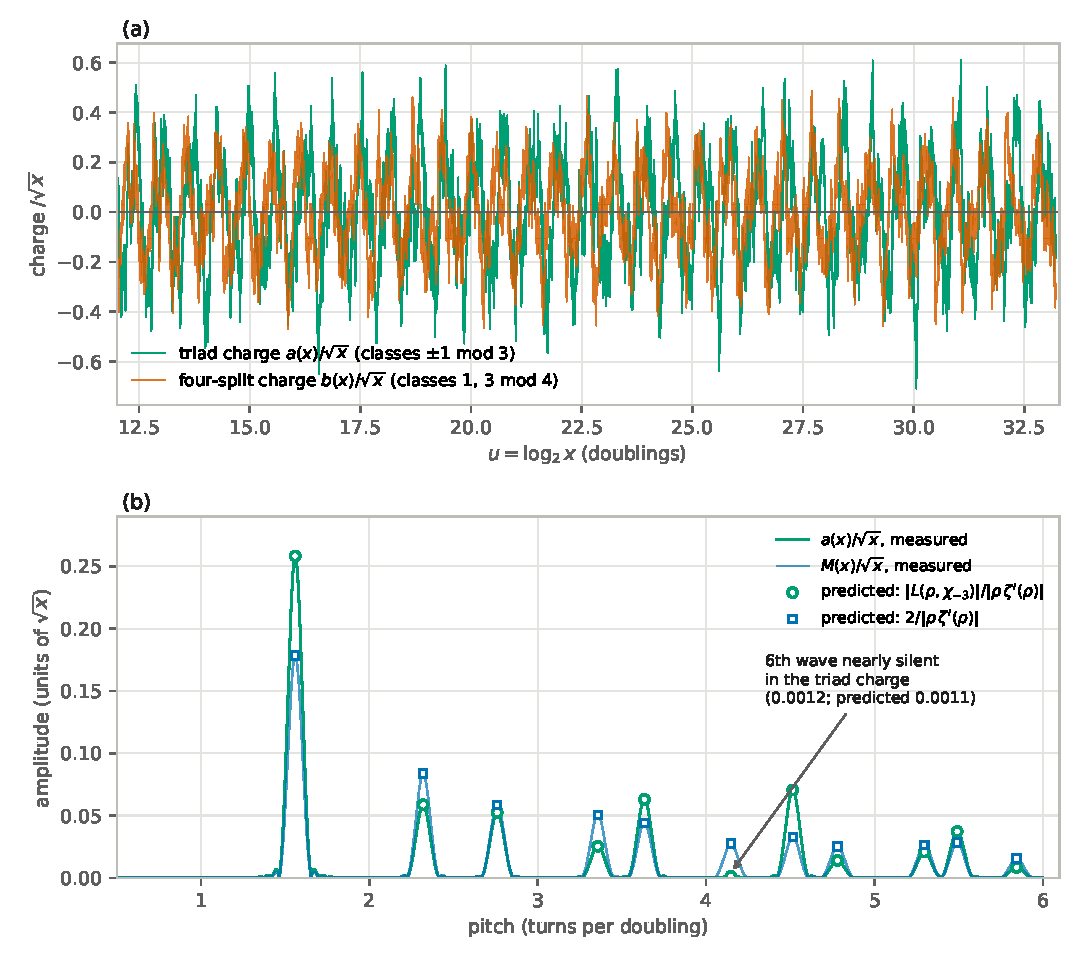
\includegraphics[width=0.92\textwidth]{fig1_triad_charge.pdf}
\caption{(a) The triad charge $a(x)/\sqrt x$ (classes $\pm1\bmod3$) and the four-split charge $b(x)/\sqrt x$ (classes $1,3\bmod4$) for $2^{12}\le x\le10^{10}$, from the exact sieve. (b) Amplitude spectra in doublings of $a(x)/\sqrt x$ and $M(x)/\sqrt x$, with the amplitudes $|L(\rho,\chi_{-3})|/|\rho\zeta'(\rho)|$ (circles) and $2/|\rho\zeta'(\rho)|$ (squares) of \eqref{eq:amps} at the pitches of the zeros. The sixth wave is nearly silent in the triad charge.}\label{fig:triad}
\end{figure}

\section{Prime gaps with the prime squares}\label{sec:gaps}

\begin{proof}[Proof of \cref{mt:gaps}]
(i) Let $n\in[p,pp')$ be composite with no prime factor below $p$, and write $n=q_1q_2\cdots q_j$ with $j\ge2$ and $p\le q_1\le q_2\le\dots$. If $q_2\ge p'$ then $n\ge pp'$, which is excluded; so $q_1=q_2=p$, the only prime in $[p,p')$. If $j\ge3$ then $n\ge p^3>pp'$, because $p^2\ge2p>p'$ by Bertrand's postulate. Hence $n=p^2$, which lies in the window since $p<p'$. Conversely every prime in $[p,pp')$ and $p^2$ have no prime factor below $p$.
(ii) An odd square is $\equiv1\pmod8$, and a square prime to $3$ is $\equiv1\pmod3$.
(iii) For integers $\equiv\pm1\pmod6$, a gap $\equiv2\pmod6$ leads from the class $-1$ to the class $+1$, a gap $\equiv4$ from $+1$ to $-1$, and a gap $\equiv0$ stays in its class. The crossings therefore alternate in direction, and the two counts differ by $[n_{\mathrm{last}}\equiv1]-[n_{\mathrm{first}}\equiv1]\in\{-1,0,1\}$. By (ii) every prime square $\ge25$ is $\equiv1\pmod6$.
\end{proof}

\begin{corollary}[each square opens the next wheel]\label{cor:wheel}
Let $W_p=\prod_{q<p}q$. On $[p,pp')$ the gaps between consecutive members of the primes together with $p^2$ are the gaps of the wheel of integers prime to $W_p$. The least composite member of this wheel is $p^2$, and the next is $pp'$.
\end{corollary}

For $p=5$ the window is $[5,35)$ and the wheel is that of $6$: the numbers $5,7,11,13,17,19,23,25,29,31$ have gaps $2,4,2,4,\dots$. For $p=7$ the window is $[7,77)$ and the wheel is that of $30$; for $p=11$ it is $[11,143)$ and the wheel of $210$. We have checked the window law directly through $p=19$. The wheel of $30$ is symmetric about $30$, since $\gcd(n,30)=\gcd(60-n,30)$: its members in $(0,60)$ lie at the distances $1,7,11,13,17,19,23,29$ from $30$ on both sides, and $49=60-11$, $59=60-1$. With $49$ inserted, the gaps from $7$ to $67$ are the gaps of the wheel of $30$, namely $4,2,4,2,4,6,2,6$, twice.

\subsection{Gaps and classes up to 61}

From $5$ to $59$ the gaps of the primes are
\[
2,4,2,4,2,4,6,2,6,4,2,4,6,6,
\]
and with $25$ and $49$ inserted they are
\[
2,4,2,4,2,4,2,4,2,6,4,2,4,2,4,6 .
\]
\Cref{tab:triads} lists the ten triads $6k-1,6k,6k+1$ up to $61$. Without the squares the classes $6k-1$ and $6k+1$ hold $9$ and $7$ primes, and the four gaps of length $6$ ($23\to29$, $31\to37$, $47\to53$, $53\to59$) pass over $25$, $35$, $49$ and $55$: three times over the class $+1$ and once over the class $-1$. With the squares inserted the two classes stand $9:9$, each with exactly one composite not a square, $35=5\cdot7$ and $55=5\cdot11$, and the two remaining gaps of length $6$ pass over these two, one in each class. The gaps $\equiv2$ and $\equiv4\pmod6$ number $5$ and $5$ without the squares and $7$ and $7$ with them.

\begin{table}[!htbp]\centering\small
\begin{tabular}{@{}rccc|rccc@{}}\toprule
$k$ & $6k-1$ & $6k$ & $6k+1$ & $k$ & $6k-1$ & $6k$ & $6k+1$\\\midrule
$1$ & $5$ & $6$ & $7$ & $6$ & $35=5\cdot7$ & $36$ & $37$\\
$2$ & $11$ & $12$ & $13$ & $7$ & $41$ & $42$ & $43$\\
$3$ & $17$ & $18$ & $19$ & $8$ & $47$ & $48$ & $49=7^2$\\
$4$ & $23$ & $24$ & $25=5^2$ & $9$ & $53$ & $54$ & $55=5\cdot11$\\
$5$ & $29$ & $30$ & $31$ & $10$ & $59$ & $60$ & $61$\\\bottomrule
\end{tabular}
\caption{The ten triads up to $61$. The class $6k-1$ holds nine primes and the composite $35$; the class $6k+1$ holds seven primes, the two squares $25$ and $49$, and the composite $55$.}\label{tab:triads}
\end{table}

\subsection{Beyond 61}

Up to $10^8$ the gaps between consecutive primes from $5$ on number $1{,}616{,}470$ ($\equiv2\bmod6$), $1{,}616{,}470$ ($\equiv4$) and $2{,}528{,}512$ ($\equiv0$). \Cref{tab:classcount} compares the two classes with the prime squares counted at weight $0$, $1$ and $\frac12$. At weight $1$ the class $6k+1$ pulls ahead as the squares accumulate; at weight $\frac12$ the difference stays within the oscillation carried by the zeros of $L(s,\chi_{-3})$, of scale $\sqrt x/\log x$, which is $543$ at $10^8$. \Cref{sec:lean} explains the weight $\frac12$.

\begin{table}[!htbp]\centering\small
\begin{tabular}{@{}rrrrrrr@{}}\toprule
$x$ & $\pi(x;6,5)$ & $\pi(x;6,1)$ & squares & difference & squares at weight $1$ & squares at weight $\frac12$\\\midrule
$61$ & $9$ & $7$ & $2$ & $2$ & $0$ & $1$\\
$100$ & $12$ & $11$ & $2$ & $1$ & $-1$ & $0$\\
$10^3$ & $86$ & $80$ & $9$ & $6$ & $-3$ & $1.5$\\
$10^4$ & $616$ & $611$ & $23$ & $5$ & $-18$ & $-6.5$\\
$10^5$ & $4{,}806$ & $4{,}784$ & $63$ & $22$ & $-41$ & $-9.5$\\
$10^6$ & $39{,}265$ & $39{,}231$ & $166$ & $34$ & $-132$ & $-49$\\
$10^7$ & $332{,}383$ & $332{,}194$ & $444$ & $189$ & $-255$ & $-33$\\
$10^8$ & $2{,}880{,}936$ & $2{,}880{,}517$ & $1{,}227$ & $419$ & $-808$ & $-194.5$\\\bottomrule
\end{tabular}
\caption{The classes $6k-1$ and $6k+1$ of the primes up to $x$, the number of prime squares $p^2\le x$ with $p\ge5$ (all in the class $6k+1$), and $\pi(x;6,5)-\pi(x;6,1)-w\cdot\#\text{squares}$ for $w=0,1,\frac12$.}\label{tab:classcount}
\end{table}

\section{The squares carry the lean}\label{sec:lean}

\begin{proof}[Proof of \cref{mt:wheel}]
(i) For $\sigma>1$, $\sum_{(n,W)=1}n^{-s}=\sum_nn^{-s}\sum_{d\mid(n,W)}\mu(d)=\sum_{d\mid W}\mu(d)d^{-s}\zeta(s)$. The finite product $\prod_{q\mid W}(1-q^{-s})$ is entire and has no zeros in $\sigma>0$, because $|q^{-s}|<1$ there. Likewise $\Phi_W(x)=\sum_{d\mid W}\mu(d)\lfloor x/d\rfloor=x\sum_{d\mid W}\mu(d)/d-\sum_{d\mid W}\mu(d)\fr{x/d}$, with $\sum_{d\mid W}\mu(d)/d=\varphi(W)/W$; each $\fr{x/d}$ has period $d\mid W$, and $W$ has $2^{\nu(W)}$ divisors.
(ii) $\log\zeta(s)=-\sum_p\log(1-p^{-s})=\sum_p\sum_kp^{-ks}/k$, and $J$ jumps by $1/k$ at each $p^k$. Then $\sum_k\mu(k)k^{-1}J(x^{1/k})=\sum_{k,j}\mu(k)(kj)^{-1}\pi(x^{1/kj})=\sum_n\pi(x^{1/n})n^{-1}\sum_{k\mid n}\mu(k)=\pi(x)$, all sums being finite.
(iii) By definition $\pi(x)=J(x)-\frac12\pi(\sqrt x)-\sum_{k\ge3}\pi(x^{1/k})/k$, the last sum is $O(x^{1/3})$, and $\pi(\sqrt x)=\li(\sqrt x)+O(\sqrt x\,\e^{-c\sqrt{\log x}})$ by the prime number theorem \cite[Ch.~18]{Davenport}. The formula for $J$ is Riemann's \cite{Riemann}, proved by von Mangoldt \cite{vonMangoldt}.
(iv) $\zeta(2s)/\zeta(s)=\zeta(2s)\cdot\zeta(s)^{-1}$ gives $\lambda(n)=\sum_{d^2\mid n}\mu(n/d^2)$, so $L(x)=\sum_{d^2m\le x}\mu(m)=\sum_{d\le\sqrt x}M(x/d^2)$.
(v) The left side is $\sum_{k\ge2}\sum_{p^k\le x}\log p\,\bigl([p^k\equiv1]-[p^k\equiv5]\bigr)\pmod6$. Powers of $2$ and $3$ are not prime to $6$. For $p\ge5$, $p^2\equiv1\pmod6$ by \cref{mt:gaps}(ii), so $k=2$ gives $\sum_{5\le p\le\sqrt x}\log p=\theta(\sqrt x)-\log6$, and the terms $k\ge3$ total at most $\sum_{3\le k\le\log_2x}\theta(x^{1/k})=O(x^{1/3}\log x)$.
\end{proof}

\paragraph{Three weights for one square.} Since $\sqrt{p^2}=p$, the prime square sits on its own square-root horizon, and three counts weigh it differently. The wheel of modulus $W_p$ counts $p^2$ as a member, with weight $1$ (\cref{cor:wheel}); the primes leave it out, with weight $0$; the logarithm of the Euler product counts it with weight $\frac12$ (\cref{mt:wheel}(ii)). By \cref{mt:wheel}(i) every wheel series vanishes at every zero of $\zeta$, yet its count carries no wave: its error is bounded and periodic, and for the wheel of $\prod_{p\le37}p$ the spectrum in doublings of the error divided by $\sqrt x$ has amplitude at most $0.0018$ at every pitch in $[0.3,6]$ up to $10^{10}$ \cite{S10}. The zeros become waves only through the logarithm, which turns each of them into a pole of $\zeta'/\zeta$, and the count that carries these waves with no term of order $\sqrt x/\log x$ is $J$, in which the squares have weight $\frac12$. By \cref{mt:wheel}(iii), $\pi(x)-\li(x)$ contains in addition $-\frac12\li(\sqrt x)\sim-\sqrt x/\log x$: the lean of $\pi$ against $\li$ is the square term. In the same way $L(x)-M(x)=\sum_{d\ge2}M(x/d^2)$ carries the constant $1/\zeta(\frac12)$ of the pole of $\zeta(2s)$ at $s=\frac12$ (\cref{mt:reverse}(i)), and by \cref{mt:wheel}(v) the difference $\theta(x;6,1)-\theta(x;6,5)$ carries $-\theta(\sqrt x)\sim-\sqrt x$, while $\psi(x;6,1)-\psi(x;6,5)=\psi(x,\chi_{-3})+O(\log x)$ is, by its explicit formula \cite[Ch.~19]{Davenport}, a sum of waves from the zeros of $L(s,\chi_{-3})$. This is the mechanism of Chebyshev's bias identified by Rubinstein and Sarnak \cite{RubinsteinSarnak}.

\subsection{Measurements}

The counts to $10^{10}$ of \cite{S10} give $\pi$, $\li$, $M$, $L$, $\theta$ and $\psi$ in the classes modulo $6$ exactly. On the grid $u=12+0.001j$, $2^{12}\le x\le10^{10}$ ($21{,}220$ points), \cref{tab:lean} compares four counts with the squares left out and with the squares at weight $\frac12$.

\begin{table}[!htbp]\centering\small
\setlength{\tabcolsep}{4pt}
\begin{tabular}{@{}llrrr@{}}\toprule
count & squares & mean & time above $0$ & sign changes\\\midrule
$(\pi(x)-\li(x))\log x/\sqrt x$ & left out & $-1.364$ & $0.000$ & $0$\\
$(J(x)-\li(x)+\log2)\log x/\sqrt x$ & weight $\frac12$ & $+0.0013$ & $0.501$ & $1816$\\[2pt]
$L(x)/\sqrt x=\sum_dM(x/d^2)/\sqrt x$ & $d^2$-multiples in & $-0.6834$ & $0.000$ & $0$\\
$M(x)/\sqrt x$ & $d^2$-multiples out & $-0.0046$ & $0.484$ & $826$\\[2pt]
$(\theta(x;6,1)-\theta(x;6,5))/\sqrt x$ & left out & $-0.973$ & $0.001$ & $14$\\
$(\psi(x;6,1)-\psi(x;6,5))/\sqrt x$ & weight $\frac12$ & $-0.0039$ & $0.502$ & $1273$\\[2pt]
$(\pi(x;6,5)-\pi(x;6,1))\log x/\sqrt x$ & left out & $+1.157$ & $1.000$ & $0$\\
$(\pi(x;6,5)-\pi(x;6,1)-\frac12\pi_\square(x))\log x/\sqrt x$ & weight $\frac12$ & $+0.031$ & $0.526$ & $1408$\\\bottomrule
\end{tabular}
\caption{The lean of four prime counts over $2^{12}\le x\le10^{10}$: mean over the grid, fraction of the grid where the count is positive, and number of sign changes on the grid. In $\psi$ the prime power $p^k$ has weight $\log p=\frac1k\log p^k$, so its squares enter with weight $\frac12$ relative to their position; $\pi_\square(x)=\#\{p\ge5:p^2\le x\}$.}\label{tab:lean}
\end{table}

\paragraph{The balancing weight.} For $\pi_w(x)=\pi(x)+w\,\pi(\sqrt x)+\sum_{k\ge3}\pi(x^{1/k})/k$, so that $\pi_0$ omits the squares and $\pi_{1/2}=J$, the mean of $(\pi_w(x)-\li(x)+\log2)\log x/\sqrt x$ over the grid is linear in $w$: it is $-1.147$ at $w=0$ and $+1.150$ at $w=1$, and it vanishes at $w^*=0.4994$, with $0.4992$ and $0.4997$ on the two halves of the range.
For the classes, the weight $w$ that centres $\pi(x;6,5)-\pi(x;6,1)-w\,\pi_\square(x)$ is $0.514$ ($0.518$ and $0.509$ on the two halves).

\paragraph{The waves are unchanged.} The amplitudes of $(J(x)-\li(x))\log x/\sqrt x$ at the first eight zeros are $0.1419$, $0.0954$, $0.0798$, $0.0658$, $0.0609$, $0.0532$, $0.0492$ and $0.0462$, against $2/|\rho|=0.1414$, $0.0951$, $0.0799$, $0.0657$, $0.0607$, $0.0532$, $0.0489$ and $0.0462$, and $\pi-\li$ carries the same waves. The square weight moves the centre of the count and nothing else.

\paragraph{The Liouville lean.} $L(x)-M(x)=\sum_{d\ge2}M(x/d^2)$ has mean $-0.6788\sqrt x$ over the grid, against $1/\zeta(\frac12)=-0.6848$; it holds almost the whole lean of $L$, while $M$ itself is centred. Tanaka \cite{Tanaka} found $L(x)\le0$ for $2\le x<906{,}150{,}257$, answering a question of Pólya \cite{Polya}; in \cref{tab:lean} the same count with its square multiples removed is $M$, which changes sign $826$ times on the grid. Likewise $\pi(x)<\li(x)$ at every grid point, although $\pi(x)-\li(x)$ changes sign infinitely often \cite{Littlewood14}, while $J(x)-\li(x)+\log2$ changes sign $1816$ times.

\begin{figure}[!htbp]\centering
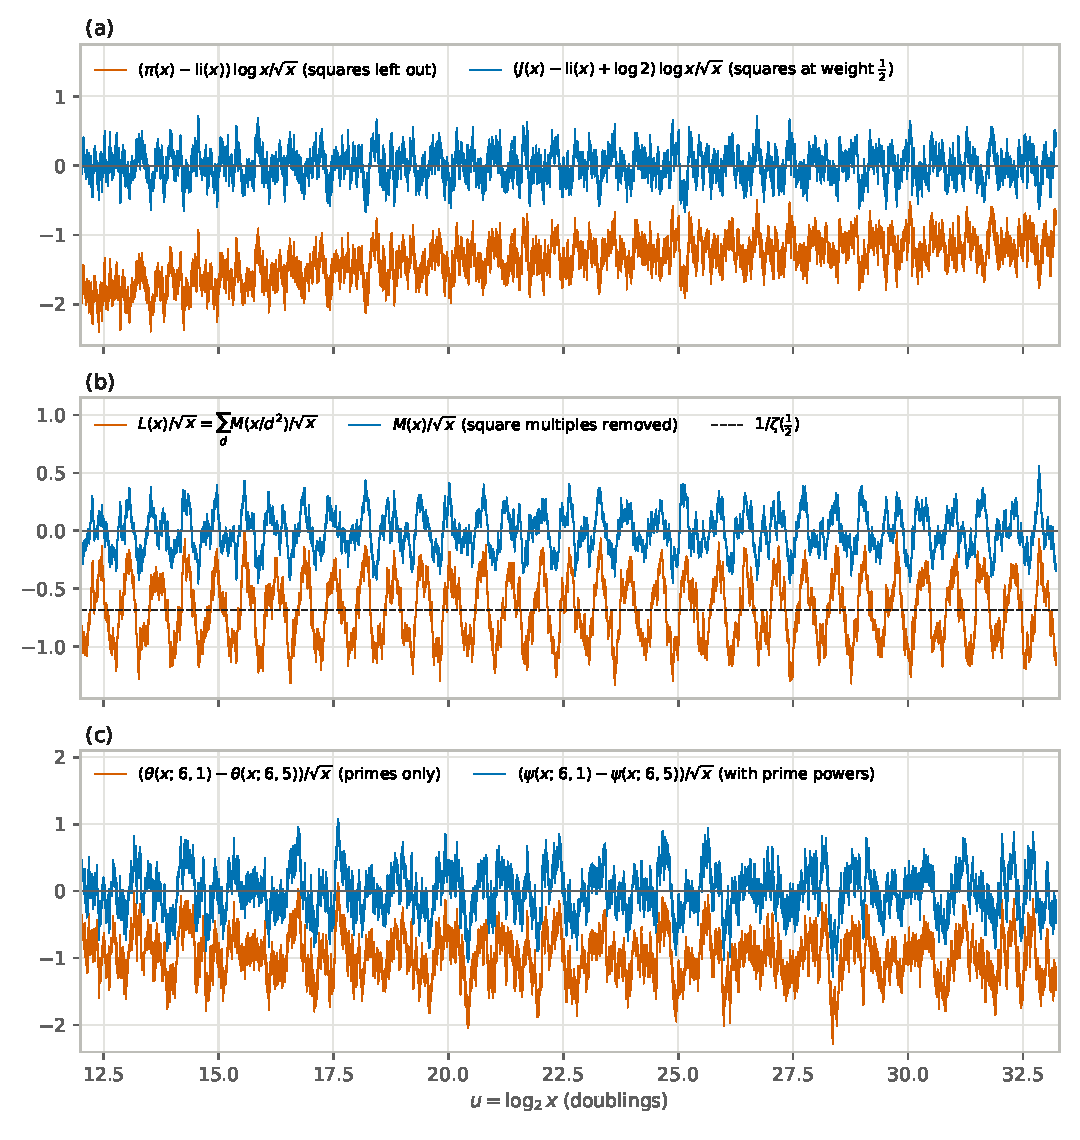
\includegraphics[width=0.92\textwidth]{fig2_square_lean.pdf}
\caption{The squares carry the lean, $2^{12}\le x\le10^{10}$. (a) $(\pi(x)-\li(x))\log x/\sqrt x$ and $(J(x)-\li(x)+\log2)\log x/\sqrt x$. (b) $L(x)/\sqrt x$ and $M(x)/\sqrt x$, with $1/\zeta(\frac12)$ dashed. (c) $(\theta(x;6,1)-\theta(x;6,5))/\sqrt x$ and $(\psi(x;6,1)-\psi(x;6,5))/\sqrt x$. In each panel the count with the squares at weight $\frac12$ is centred and carries the same waves.}\label{fig:lean}
\end{figure}

\section{The square-root horizon}\label{sec:horizon}

We call $\sigma=\frac12$ the square-root horizon: it is the line where the squares series $\sum_pp^{-2\sigma}$, and with it the part of $\log\zeta$ carried by the prime squares and higher powers, stops converging. Write $P(s)=\sum_pp^{-s}$ for $\sigma>1$, so that $\log\zeta=P+S$.

\begin{proof}[Proof of \cref{mt:horizon}]
(i) For $\sigma>\frac12$, $\sum_p\sum_{k\ge2}|p^{-ks}|/k\le\sum_pp^{-2\sigma}(1-p^{-\sigma})^{-1}<\infty$, uniformly on compact sets, so $S$ is analytic and $E=\e^S$ is analytic and zero-free there. For $\sigma>1$, $\log\zeta(s)=\sum_{m\ge1}P(ms)/m$, and Möbius inversion, justified by absolute convergence, gives
\begin{equation}\label{eq:Pinv}
P(s)=\sum_{k\ge1}\frac{\mu(k)}k\log\zeta(ks),\qquad S(s)=-\sum_{k\ge2}\frac{\mu(k)}k\log\zeta(ks).
\end{equation}
For $k\ge2$ and $\sigma>\frac12$, $|\log\zeta(ks)|\le\log\zeta(k\sigma)\le\zeta(k\sigma)-1\ll2^{-k\sigma}$, so the second series converges to an analytic function of $\sigma>\frac12$, which is $S$ there. Since $E$ has neither zeros nor poles in $\sigma>\frac12$, $F=\zeta/E$ is meromorphic there with the zeros of $\zeta$ and their orders, and $F=\e^P$ for $\sigma>1$.
(ii) $\log|E(\sigma+it)|=\Re S=\sum_p\sum_{k\ge2}p^{-k\sigma}k^{-1}\cos(kt\log p)$, so, with $\theta=kt\log p$,
\[
3\log E(\sigma)+4\log|E(\sigma+it)|+\log|E(\sigma+2it)|=\sum_p\sum_{k\ge2}\frac{p^{-k\sigma}}k\,(3+4\cos\theta+\cos2\theta),
\]
an absolutely convergent series of terms $\frac{p^{-k\sigma}}k\cdot2(1+\cos\theta)^2\ge0$.
(iii) Since $\mu(2)=-1$, \eqref{eq:Pinv} gives $2S(s)=\log\zeta(2s)-2R(s)$ with $R(s)=\sum_{k\ge3}\mu(k)k^{-1}\log\zeta(ks)$. For $k\ge3$ and $\sigma>\frac13$, $\Re(ks)>1$ and the bound of (i) makes $R$ analytic in $\sigma>\frac13$. Hence $E(s)^2=\zeta(2s)\e^{-2R(s)}$ continues meromorphically to $\sigma>\frac13$. The factor $\e^{-2R}$ has no zeros or poles; $\zeta(2s)$ has its only pole at $s=\frac12$ and no zeros with $\Re(2s)\ge1$ \cite[\S3.3]{Titchmarsh}. Since $\zeta(\frac12)=-1.4603\ldots\ne0$, $F(s)^2=\zeta(s)^2\e^{2R(s)}/\zeta(2s)$ has a simple zero at $s=\frac12$. For real $\sigma\to\frac12+$, $\zeta(2\sigma)=(2\sigma-1)^{-1}+\gamma_E+O(2\sigma-1)$ \cite[\S2.1]{Titchmarsh}, so $\log E(\sigma)+\frac12\log(2\sigma-1)=-R(\sigma)+O(2\sigma-1)\to-R(\frac12)=C_E$, and $\log|F(\sigma)|-\frac12\log(2\sigma-1)=\log|\zeta(\sigma)|-\bigl(\log E(\sigma)+\frac12\log(2\sigma-1)\bigr)\to\log|\zeta(\frac12)|-C_E$.
(iv) Let $\rho=\frac12+i\gamma$ have multiplicity $m$. As $\sigma\to\frac12+$, $3\log|\zeta(\sigma)|\to3\log|\zeta(\frac12)|$, $\log|\zeta(\sigma+2i\gamma)|$ tends to $\log|\zeta(\frac12+2i\gamma)|$ or to $-\infty$, and $4\log|\zeta(\sigma+i\gamma)|=4m\log(\sigma-\frac12)+O(1)\to-\infty$. So $Q_\zeta(\sigma,\gamma)\to-\infty$. By (iii), $3\log E(\sigma)=\frac32\log\frac1{2\sigma-1}+O(1)$, while $\log|E(\sigma+i\gamma)|$ and $\log|E(\sigma+2i\gamma)|$ stay bounded, because $E^2$ is analytic and zero-free at $\frac12+i\gamma$ and $\frac12+2i\gamma$; hence $Q_F=Q_\zeta-Q_E\to-\infty$ as well.
\end{proof}

\begin{remark}[the half-order zero is the square lean]\label{rem:halforder}
The expansion $P(s)=\log\zeta(s)-\frac12\log\zeta(2s)-\frac13\log\zeta(3s)-\frac15\log\zeta(5s)+\frac16\log\zeta(6s)-\dots$ of \eqref{eq:Pinv} is, term by term, Riemann's expansion $\pi(x)=J(x)-\frac12J(\sqrt x)-\frac13J(x^{1/3})-\dots$ of \cref{mt:wheel}(ii). The term $-\frac12\log\zeta(2s)$, which near $s=\frac12$ is $\frac12\log(2s-1)+O(1)$, is the half-order zero of $F=\e^P$ at the horizon, and in the count it is $-\frac12J(\sqrt x)=-\frac12\li(\sqrt x)+\dots$, the lean of $\pi$ against $\li$ measured in \cref{sec:lean}. The half-order pole of $E$ at $s=\frac12$ is the same square term seen from the squares part.
\end{remark}

\begin{remark}[edge and horizon]\label{rem:edge}
For $\zeta$ itself the squared pair is nonnegative for $\sigma>1$, $\zeta(\sigma)^3|\zeta(\sigma+it)|^4|\zeta(\sigma+2it)|\ge1$ \cite{Mertens}, \cite[\S3.3]{Titchmarsh}, from the identity $3+4\cos\theta+\cos2\theta=2(1+\cos\theta)^2\ge0$ \cite[(3.3.1)]{Titchmarsh}, which gives $\zeta(1+it)\ne0$ and, by the functional equation, $\zeta(it)\ne0$. The inequality for $\zeta$ splits as $Q_\zeta=Q_E+Q_F$: the prime part $Q_F=\sum_pp^{-\sigma}\cdot2(1+\cos(t\log p))^2\ge0$ holds for $\sigma>1$, and the squares part $Q_E\ge0$ holds all the way down to the horizon by \cref{mt:horizon}(ii). The zeros of $\zeta$ in $\sigma>\frac12$ are exactly those of the prime factor $F$ (\cref{mt:horizon}(i)). At the horizon the squares part has a half-order pole and the prime factor a half-order zero, and by \cref{mt:horizon}(iv) the squared pair of $\zeta$ and of $F$ is negative arbitrarily close to the horizon at the height of every zero on it.
\end{remark}

\subsection{Measurements}

\paragraph{The squares part.} By \eqref{eq:Pinv}, $\log|E(s)|=-\sum_{k\ge2}\mu(k)k^{-1}\log|\zeta(ks)|$ involves $\zeta$ only in $\sigma>1$. At $200$ random points with $\frac12<\sigma<1$ and $1<t<61$ the squared pair $Q_E$ has minimum $0.3355$. \Cref{tab:halforder} shows the half-order limits of \cref{mt:horizon}(iii).

\begin{table}[!htbp]\centering\small
\begin{tabular}{@{}lrrrrrrr@{}}\toprule
$\sigma$ & $0.6$ & $0.55$ & $0.51$ & $0.505$ & $0.501$ & $0.5001$ & limit\\\midrule
$\log E(\sigma)+\frac12\log(2\sigma-1)$ & $0.29424$ & $0.31979$ & $0.35315$ & $0.35842$ & $0.36285$ & $0.36387$ & $0.36399$\\
$\log|F(\sigma)|-\frac12\log(2\sigma-1)$ & $0.37495$ & $0.19824$ & $0.05258$ & $0.03374$ & $0.01852$ & $0.01507$ & $0.01469$\\\bottomrule
\end{tabular}
\caption{The half-order pole of the squares part $E$ and the half-order zero of the prime factor $F=\zeta/E$ at $s=\frac12$. The two limits add up to $\log|\zeta(\frac12)|=0.37868$.}\label{tab:halforder}
\end{table}

\paragraph{The reach of the squared pair of $\zeta$.} For a zero $\frac12+i\gamma$ let its reach be the largest $\sigma\in[0.5005,1]$ at which $\min_{|t-\gamma|\le0.3}Q_\zeta(\sigma,t)<0$. At the first $41$ zeros and every $25$th zero after them, $138$ zeros in all up to height $3000$, the reach lies between $0.546$ and $0.847$ (\cref{tab:reach}, \cref{fig:reach}). For the prime factor alone the reach at the first twelve zeros is $0.888$, $0.862$, $0.855$, $0.869$, $0.848$, $0.798$, $0.837$, $0.806$, $0.852$, $0.856$, $0.775$ and $0.773$. Above the reach the squared pair of $\zeta$ is nonnegative at the sampled points of the window, and at such points $\zeta$ has no zero; below it the band of negative values extends down to the zero on the horizon, as \cref{mt:horizon}(iv) requires.

\begin{table}[!htbp]\centering\small
\begin{tabular}{@{}lrrrrrr@{}}\toprule
height of the zero & $<50$ & $50$--$100$ & $100$--$300$ & $300$--$1000$ & $1000$--$2000$ & $2000$--$3000$\\\midrule
zeros & $10$ & $19$ & $15$ & $21$ & $35$ & $38$\\
mean reach & $0.802$ & $0.761$ & $0.747$ & $0.727$ & $0.711$ & $0.693$\\
largest reach & $0.839$ & $0.818$ & $0.837$ & $0.847$ & $0.845$ & $0.825$\\\bottomrule
\end{tabular}
\caption{Reach of the negative band of the squared pair $Q_\zeta$ beside the zeros of $\zeta$.}\label{tab:reach}
\end{table}

\begin{figure}[!htbp]\centering
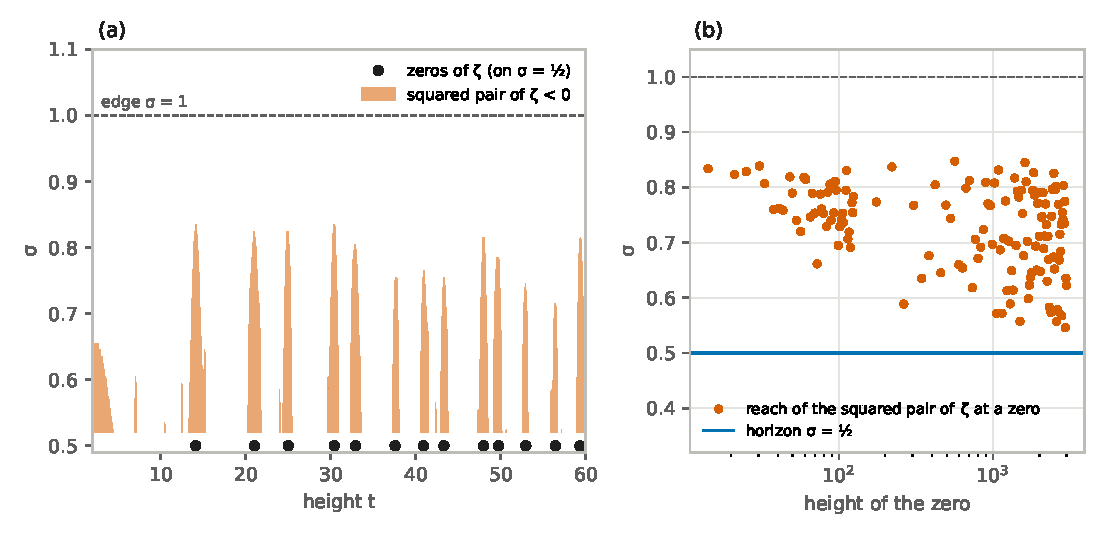
\includegraphics[width=0.95\textwidth]{fig3_squared_pair_reach.pdf}
\caption{(a) The region $\frac12<\sigma\le1.1$, $2\le t\le60$ where the squared pair $Q_\zeta$ is negative, and the zeros of $\zeta$ on $\sigma=\frac12$. (b) The reach of the negative band at $138$ zeros up to height $3000$. The squares part satisfies $Q_E\ge0$ everywhere above the horizon.}\label{fig:reach}
\end{figure}

\section{The prime term at every height}\label{sec:phases}

By \cref{mt:horizon} every zero of $\zeta$ in $\sigma>\frac12$ is a zero of the prime factor $F$, whose logarithm is the prime term $P(s)=\sum_pp^{-s}$ for $\sigma>1$. At height $t$ the prime term is the sum of the unit vectors $p^{-it}=\e^{-it\log p}$ weighted by $p^{-\sigma}$, and its phases $t\log p$ behave as independent in the sense of \cref{mt:phases}(i): any finitely many of them are jointly equidistributed.

\begin{proof}[Proof of \cref{mt:phases}\textup{(i)--(iii)}]
(i) By unique factorisation the numbers $\log p$ are linearly independent over $\mathbb Q$: an integer relation $\sum a_p\log p=0$ gives $\prod p^{a_p}=1$, so every $a_p=0$. Hence for every nonzero integer vector $(k_p)_{p\le y}$, $\sum k_p\log p\ne0$ and $\frac1T\int_0^T\e^{it\sum_pk_p\log p}\dd t\to0$, and Weyl's criterion \cite{Weyl} gives the equidistribution of $t(\log p/2\pi)_{p\le y}$ modulo $1$; this is Kronecker's theorem in Weyl's form \cite[Ch.~XXIII]{HardyWright}.
(ii) $\mathbb E\,\e^{i(\vartheta_p-\vartheta_q)}=[p=q]$ gives the variance. For $\sigma>\frac12$ the independent terms have mean $0$ and summable variances, so the series converges almost surely \cite{KhintchineKolmogoroff}, \cite[Theorem 2.5.6]{Durrett}. For $\sigma\le\frac12$ the real parts $p^{-\sigma}\cos\vartheta_p$ are independent, have mean $0$, are bounded by $1$ and have variances $\frac12p^{-2\sigma}$ with divergent sum, so by Kolmogorov's three-series theorem with truncation level $1$ \cite[Theorem 2.5.8]{Durrett} their sum does not converge almost surely; by Kolmogorov's zero-one law it diverges almost surely.
(iii) Let $Z_y=\prod_{p\le y}(1-p^{-\sigma}\e^{i\vartheta_p})^{-1}=\prod_{p\le y}\sum_{j\ge0}p^{-j\sigma}\e^{ij\vartheta_p}$. Each factor has mean $1$ and mean square $\sum_jp^{-2j\sigma}=(1-p^{-2\sigma})^{-1}$, so by independence $\mathbb E|Z_y|^2=\prod_{p\le y}(1-p^{-2\sigma})^{-1}$. For $y<y'$ let $Z_{y,y'}=Z_{y'}/Z_y$, which is independent of $Z_y$ and has mean $1$; then $\mathbb E|Z_{y'}-Z_y|^2=\mathbb E|Z_y|^2\bigl(\mathbb E|Z_{y,y'}|^2-1\bigr)\le\zeta(2\sigma)\bigl(\prod_{y<p\le y'}(1-p^{-2\sigma})^{-1}-1\bigr)\to0$. So $Z_y$ converges in mean square, and $\mathbb E|Z_\sigma|^2=\lim\mathbb E|Z_y|^2=\zeta(2\sigma)$. Also $\log Z_y=\sum_{p\le y}\bigl(p^{-\sigma}\e^{i\vartheta_p}+O(p^{-2\sigma})\bigr)$ converges almost surely by (ii), so $Z_y$ converges almost surely to $\exp(\lim\log Z_y)\ne0$, which is $Z_\sigma$.
\end{proof}

Part (iv) consists of classical theorems: the mean square is Theorem 7.2 of \cite{Titchmarsh}, due to Hardy and Littlewood; $N(\sigma,T)=O(T)$ is Theorem 9.15(A) of \cite{Titchmarsh}, due to Bohr and Landau \cite{BohrLandau}; the bound $N(\sigma,T)=O(T^{1-(\sigma-\frac12)/4}\log T)$ is Theorem 9.19(C) of \cite{Titchmarsh}, due to Selberg \cite{Selberg46}; and the limiting distribution is due to Bohr and Jessen \cite{BohrJessen1,BohrJessen2}. Since $N(T)\sim\frac T{2\pi}\log T$, the zeros with $\beta>\sigma$ are a proportion $O(1/\log T)$ of the zeros up to height $T$, for every fixed $\sigma>\frac12$.

The squares series appears twice. In the model, the variance of the prime term is $\sum_pp^{-2\sigma}$ and the mean square of the Euler product is $\zeta(2\sigma)=\sum_nn^{-2\sigma}$ (\cref{mt:phases}(ii),(iii)); for $\zeta$ itself, the mean square over heights is the same $\zeta(2\sigma)$ (\cref{mt:phases}(iv)). Both are finite exactly for $\sigma>\frac12$. For $\frac12<\sigma<1$ the mean square has the second main term
\begin{equation}\label{eq:matsumoto}
\int_0^T|\zeta(\sigma+it)|^2\dd t=\zeta(2\sigma)T+\frac{(2\pi)^{2\sigma-1}\zeta(2-2\sigma)}{2-2\sigma}T^{2-2\sigma}+\Delta_\sigma(T),
\end{equation}
where Matsumoto \cite{Matsumoto} proves $\Delta_\sigma(T)=O(T^{1/(1+4\sigma)}\log^2T)$ for $\frac12<\sigma<\frac34$.

\subsection{Measurements}

At $6000$ heights drawn uniformly from $[5000,6000]$ we computed $\zeta(\sigma+it)$ for $\sigma=0.6,0.7,0.8$. The model value is $\log|Z_\sigma|$ with the primes up to $10^6$ and independent uniform phases, plus a Gaussian term with the variance $\frac12\sum_{p>y}p^{-2\sigma}\approx y^{1-2\sigma}/(2(2\sigma-1)\log y)$, $y=10^6$, of the omitted primes; $6000$ model values were drawn for each $\sigma$. \Cref{tab:values} and \cref{fig:values} compare the two.

\begin{table}[!htbp]\centering\small
\begin{tabular}{@{}lccccccc@{}}\toprule
$\sigma$ & mean $|\zeta|^2$ & $\zeta(2\sigma)$ & by \eqref{eq:matsumoto} & sd of $\log|\zeta|$ & model sd & $0.1\%$ quantile & model\\\midrule
$0.6$ & $4.40$ & $5.59$ & $4.45$ & $0.882$ & $0.888$ & $-2.374$ & $-2.444$\\
$0.7$ & $3.00$ & $3.11$ & $2.98$ & $0.737$ & $0.719$ & $-1.836$ & $-1.746$\\
$0.8$ & $2.18$ & $2.29$ & $2.27$ & $0.611$ & $0.623$ & $-1.456$ & $-1.515$\\\bottomrule
\end{tabular}
\caption{The value distribution of $\zeta(\sigma+it)$ at $6000$ random heights in $[5000,6000]$ against the independent-phase model. The fourth column is the mean of $|\zeta|^2$ over $[5000,6000]$ given by the two main terms of \eqref{eq:matsumoto}.}\label{tab:values}
\end{table}

\paragraph{The deepest dips.} On the grid $t=10+0.02j$, $10\le t<3000$, the least value of $\log|\zeta(0.6+it)|$ is $-3.007$ ($|\zeta|=0.049$), at $t=1329.12$, between the close zeros $1329.044$ and $1329.205$; the model's quantile at $1/2469$, one value per zero in the range, is $-2.585$ and the least of $50{,}000$ model values, with the primes up to $10^5$, is $-2.941$. At $\sigma=0.7$ the least value is $-2.214$, at the same height, against $-1.911$ and $-2.203$. The deepest dips off the line sit beside zeros on the line, and at every computed point $|\zeta(\sigma+it)|$ is positive.

\begin{figure}[!htbp]\centering
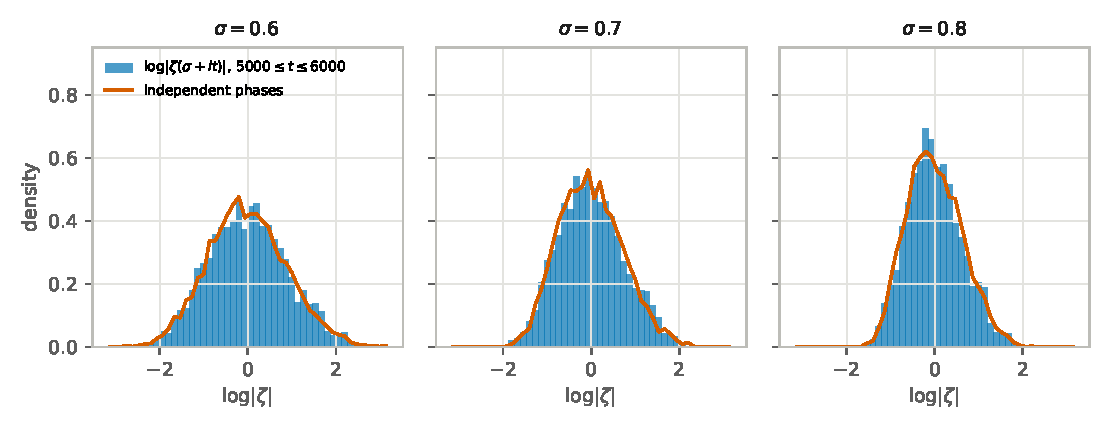
\includegraphics[width=0.98\textwidth]{fig4_value_distribution.pdf}
\caption{Distribution of $\log|\zeta(\sigma+it)|$ at $6000$ random heights $5000\le t\le6000$ for $\sigma=0.6,0.7,0.8$ (histograms), and of the independent-phase model $\log|Z_\sigma|$ (curves).}\label{fig:values}
\end{figure}

\section{The axiom of harmonic independence}\label{sec:axiom}

\begin{axiom}[harmonic independence]\label{ax:harmonic}
Harmonic independence is the absence of an integer relation. The prime waves are related only through a mechanism present in their construction. Because Unique Factorization guarantees that no integer relation exists between the primes, their wave frequencies are strictly linearly independent. A harmonic resonance between the primes beyond this explicit construction---such as a zero off the critical line---would be a relation without a mechanism.
\end{axiom}

\paragraph{The waves and their frequencies.} At height $t$ the prime $p$ enters the prime term $P(s)=\sum_pp^{-s}$ as the wave $p^{-it}=\e^{-it\log p}$, weighted by $p^{-\sigma}$, of frequency $\log p/2\pi$ in $t$; measured in doublings of $p$ it is the clock of \cref{sec:clocks}. An integer relation between the frequencies is a vector $(k_p)$ of integers, not all zero and finitely many nonzero, with $\sum_pk_p\log p=0$, that is $\prod_pp^{k_p}=1$. Unique factorisation excludes every such vector. This is the first step of the proof of \cref{mt:phases}(i), and through Kronecker's theorem in Weyl's form it makes the phases $t\log p$ of any finitely many primes jointly equidistributed on their torus: no finite set of prime waves holds a fixed phase relation over the heights, so the first part of the axiom is a theorem.

\paragraph{The mechanism in the construction.} The waves are joined in $\zeta$ by one mechanism, the Euler product $\zeta(s)=\prod_p(1-p^{-s})^{-1}$, whose expansion into $\sum_nn^{-s}$ is unique factorisation itself. The squares part $E$ and the prime factor $F$ of \cref{mt:horizon} are this mechanism divided into its terms of order two and higher and its prime term. The relations among the waves measured in this paper are made by it: the lean carried by the squares at weight $\frac12$ (\cref{mt:wheel}), the variance $\sum_pp^{-2\sigma}$ of the prime term (\cref{mt:phases}(ii)), and the half-order zero of $F$ at $s=\frac12$ that matches the half-order pole of $E$ (\cref{mt:horizon}).

\paragraph{A zero off the line.} By \cref{mt:horizon}(i) a zero $\rho=\beta+i\gamma$ with $\beta>\frac12$ is a zero of the prime factor $F$. At the height $\gamma$ it would be a relation among the prime waves weighted by $p^{-\beta}$, a resonance beyond the independence of their frequencies and beyond the relations that the Euler product supplies. The model in which the waves carry no relation at all, the independent phases of \cref{mt:phases}, has this form: there the random Euler product $Z_\sigma$ converges and is nonzero almost surely for every $\sigma>\frac12$ (\cref{mt:phases}(iii)). The axiom states as a principle that $\zeta$ admits no relation among its prime waves beyond its construction; the theorems above give its first part, the linear independence of the frequencies, and with the axiom every zero of $\zeta$ in the critical strip lies on the line $\sigma=\frac12$.

\section{The reversed pattern}\label{sec:reverse}

Reversing the sign of every prime in the Euler product gives the reversed pattern $\prod_p(1+p^{-s})^{-1}$. A zero of $\zeta$, where the forward pattern goes to $-\infty$ in logarithm, is a pole of the reversed pattern, where it goes to $+\infty$: the same pattern read in reverse order.

\begin{proof}[Proof of \cref{mt:reverse}]
(i) $(1+p^{-s})^{-1}=(1-p^{-s})(1-p^{-2s})^{-1}=\sum_{k\ge0}(-1)^kp^{-ks}$, so the product is $\zeta(2s)/\zeta(s)$ and, $\lambda$ being completely multiplicative with $\lambda(p)=-1$, equals $\sum\lambda(n)n^{-s}$ for $\sigma>1$. If $\zeta(\rho)=0$ with $\beta\ge\frac12$ then $\Re(2\rho)\ge1$, so $\zeta(2\rho)$ is finite and nonzero \cite[\S3.3]{Titchmarsh} and $\rho$ is a pole of the same order. At $s=\frac12$, $\zeta(2s)$ has a simple pole with residue $\frac12$ and $\zeta(\frac12)\ne0$.
(ii) The product $\zeta(s)\cdot\zeta(2s)/\zeta(s)=\zeta(2s)$ is the identity $\sum_{d\mid n}\lambda(d)=[n\text{ is a square}]$ \cite[Theorem 2.19]{Apostol}. Hence $\sum_{n\le x}L(x/n)=\sum_{dm\le x}\lambda(d)=\sum_{k\le x}\sum_{d\mid k}\lambda(d)$ counts the squares up to $x$.
(iii) Let $m(y)=\sum_{n\le y}\mu(n)/n$. For $y\ge1$, $\sum_{n\le y}\mu(n)\lfloor y/n\rfloor=1$, so $y\,m(y)=1+\sum_{n\le y}\mu(n)\fr{y/n}$; the term $n=1$ is $\fr y$ and the others total at most $\lfloor y\rfloor-1$ in absolute value, so $|y\,m(y)|\le y$ and $|m(y)|\le1$. Also $m(y)\to0$ \cite[Ch.~4]{Apostol}. Since $\lambda(n)=\sum_{d^2\mid n}\mu(n/d^2)$,
\[
\ell(N)=\sum_{d\le\sqrt N}\frac1{d^2}\,m\Bigl(\frac N{d^2}\Bigr),
\]
and dominated convergence, with the bound $d^{-2}$, gives $\ell(N)\to0$. Next, $\sum_{k\le x}\lambda(k)\lfloor x/k\rfloor=\sum_{n\le x}L(x/n)=\lfloor\sqrt x\rfloor$ by (ii), so $\sum_{k\le x}\lambda(k)\fr{x/k}=x\,\ell(x)-\lfloor\sqrt x\rfloor$; for $x<k\le N$, $\fr{x/k}=x/k$, which adds $x(\ell(N)-\ell(x))$. This is \eqref{eq:revsaw} for $N\ge x$, and letting $N\to\infty$ gives the series. For $0<x<1$ both sides of \eqref{eq:revsaw} vanish in the limit.
\end{proof}

In the variable $t=1/x$, with $\varsigma_k(t)=\fr{1/(kt)}$, \eqref{eq:revsaw} reads $-\sum_k\lambda(k)\varsigma_k(t)=\lfloor t^{-1/2}\rfloor$ for every $t>0$. The forward counterpart is $-\sum_k\mu(k)\varsigma_k(t)=\chi_{(0,1]}(t)$ \cite{S10}: the Möbius-weighted sawtooths rebuild the unit step, with its single jump at $t=1$, and the Liouville-weighted sawtooths rebuild the square staircase, with a jump at every $t=1/n^2$.

\paragraph{Centre and lean.} The forward pattern $\zeta(s)$ has a single pole, at its centre $s=1$. The reversed pattern has its centre pole at $s=\frac12$, made by the squares through $\zeta(2s)$. In Perron's formula for $L(x)$ this pole contributes $\sqrt x/\zeta(\frac12)=-0.6848\sqrt x$, and in that for $\ell(K)$, whose Dirichlet series is $\zeta(2+2w)/\zeta(1+w)$ at $w=s-1$, it contributes $-1/(\zeta(\frac12)\sqrt K)=0.6848/\sqrt K$. The measured mean of $L(x)/\sqrt x$ is $-0.6834$ (\cref{tab:lean}), and $\sqrt K\,\ell(K)$ leans to the positive side, while $\sqrt N\,m(N)$ is centred (\cref{tab:ell}). The other poles of the reversed pattern are the zeros of $\zeta$. Every one computed lies on the vertical line through the centre $s=\frac12$: the $2469$ below height $3000$ used here, and all below height $3\cdot10^{12}$ \cite{PT}.

\begin{table}[!htbp]\centering\small
\begin{tabular}{@{}lrrrrrrr@{}}\toprule
$K$ & $10^2$ & $10^3$ & $10^4$ & $10^5$ & $10^6$ & $10^7$ & $10^8$\\\midrule
$\sqrt K\,\ell(K)$ (reversed) & $1.0787$ & $0.9169$ & $0.4280$ & $0.4437$ & $0.8144$ & $1.0877$ & $0.9960$\\
$\sqrt K\,m(K)$ (forward) & $+0.3113$ & $+0.1395$ & $-0.2083$ & $-0.1541$ & $+0.2006$ & $+0.3210$ & $+0.2047$\\\bottomrule
\end{tabular}
\caption{Value imbalance of the first $K$ terms of the reversed and forward patterns. The reversed one leans around $-1/\zeta(\frac12)=0.6848$, the forward one around $0$.}\label{tab:ell}
\end{table}

\paragraph{Forward times reversed at a zero.} The identity of \cref{mt:reverse}(ii) holds as an identity of meromorphic functions. At a zero of $\zeta$ its left side is a zero times a pole.

\begin{proposition}[the identity at a zero]\label{prop:atzero}
Let $\rho=\beta+i\gamma$ be a zero of $\zeta$ of order $m$ with $\beta\ge\frac12$. Then:
\begin{itemize}
\item $\zeta(2s)/\zeta(s)$ has a pole of order $m$ at $\rho$;
\item the product $\zeta(s)\cdot\zeta(2s)/\zeta(s)$ is analytic at $\rho$, with the value $\zeta(2\rho)$, which is finite and nonzero;
\item for $m=1$,
\[
\operatorname*{Res}_{s=\rho}\frac{\zeta(2s)}{\zeta(s)}=\frac{\zeta(2\rho)}{\zeta'(\rho)}.
\]
\end{itemize}
In $\sigma\ge\frac12$ the squares pattern $\zeta(2s)$ has a single pole, at the centre $s=\frac12$, where $\zeta(\frac12)\ne0$.
\end{proposition}

\begin{proof}
Write $\zeta(s)=(s-\rho)^mh(s)$ with $h$ analytic near $\rho$ and $h(\rho)\ne0$. Then $\zeta(2s)/\zeta(s)=(s-\rho)^{-m}\zeta(2s)/h(s)$, and the product of the two patterns is $\zeta(2s)$. This is analytic at $\rho$ because $\Re(2\rho)\ge1$ and, $\gamma$ being nonzero, $2\rho\ne1$. Also $\zeta(2\rho)\ne0$ by \cite[\S3.3]{Titchmarsh}. For $m=1$, $h(\rho)=\zeta'(\rho)$. The only pole of $\zeta$ is at $1$, so the only pole of $\zeta(2s)$ is at $\frac12$.
\end{proof}

At every zero, the zero of the forward pattern and the pole of the reversed pattern cancel in the product. They cancel in the same way whether $\beta=\frac12$ or $\beta>\frac12$. For $\beta>\frac12$ the point $2\rho$ lies in $\sigma>1$. For $\beta=\frac12$ it lies on the edge $\sigma=1$ at height $2\gamma$, away from the pole at $1$. In both cases $\zeta(2\rho)$ is finite and nonzero. The identity therefore holds at every zero and does not by itself tell a zero on the line from a zero off it. The pole of the squares pattern sits at the centre alone, and the centre is not a zero of $\zeta$. \Cref{tab:atzero} gives the values at the first five zeros.

\begin{table}[!htbp]\centering\small
\begin{tabular}{@{}rccc@{}}\toprule
$\gamma$ & $\zeta(2\rho)=\zeta(1+2i\gamma)$ & $|\zeta(2\rho)/\zeta'(\rho)|$ & residue, direct\\\midrule
$14.134725$ & $1.836735-0.651198i$ & $2.456952$ & $2.1\times10^{-12}$\\
$21.022040$ & $0.812565+0.173883i$ & $0.730941$ & $2.7\times10^{-13}$\\
$25.010858$ & $0.444955+0.295572i$ & $0.389423$ & $1.1\times10^{-12}$\\
$30.424876$ & $0.374904+0.352748i$ & $0.394777$ & $1.4\times10^{-12}$\\
$32.935062$ & $0.789343-0.194577i$ & $0.588206$ & $3.1\times10^{-13}$\\\bottomrule
\end{tabular}
\caption{The identity of \cref{mt:reverse}(ii) at the first five zeros, computed with $30$ significant digits. The last column gives the difference between $(s-\rho)\zeta(2s)/\zeta(s)$ at $s=\rho+10^{-12}$ and $\zeta(2\rho)/\zeta'(\rho)$. At the same point the product $\zeta(s)\cdot\zeta(2s)/\zeta(s)$ differs from $\zeta(2\rho)$ by at most $2.3\times10^{-12}$; both differences are of the size of the offset. With $|1-2^{-2i\gamma}|^2$, the values $|\zeta(1+2i\gamma)|^2$ give the edge weights $|\eta(1+2i\gamma)|^2$ of \cref{sec:revNB}.}\label{tab:atzero}
\end{table}

\paragraph{Checks.} The identity \eqref{eq:revrebuild} holds exactly at $x=10$, $99$, $100$, $1000$, $12345$ and $10^5$, with values $3$, $9$, $10$, $31$, $111$ and $316$. \Cref{tab:revsaw} shows the partial sums of \eqref{eq:revsaw}; by \eqref{eq:revsaw} they equal $\lfloor\sqrt x\rfloor-x\,\ell(K)$, and the direct sums over $k\le10^4$ agree with this to all digits shown. The exact sieve gives $L(10^8)=-3884$.

\begin{table}[!htbp]\centering\small
\begin{tabular}{@{}rrrrr@{}}\toprule
$x$ & $\lfloor\sqrt x\rfloor$ & $K=10^4$ & $K=10^6$ & $K=10^8$\\\midrule
$0.7$ & $0$ & $-0.00300$ & $-0.00057$ & $-0.00007$\\
$3.9$ & $1$ & $0.98331$ & $0.99682$ & $0.99961$\\
$50.5$ & $7$ & $6.78385$ & $6.95887$ & $6.99497$\\
$99.99$ & $9$ & $8.57202$ & $8.91856$ & $8.99004$\\
$1000.3$ & $31$ & $26.71844$ & $30.18532$ & $30.90037$\\\bottomrule
\end{tabular}
\caption{The Liouville-weighted sawtooths rebuild the square staircase: $-\sum_{k\le K}\lambda(k)\fr{x/k}$ tends to $\lfloor\sqrt x\rfloor$.}\label{tab:revsaw}
\end{table}

\section{The reversed staircase criterion}\label{sec:revNB}

The criterion of Nyman and Beurling \cite{Nyman,Beurling}, in the form of Báez-Duarte \cite{BaezDuarte}, reads RH from the unit step $\chi_{(0,1]}$, which the Möbius-weighted sawtooths rebuild exactly \cite{S10}: RH holds if and only if $d_N\to0$. The reversed pattern rebuilds the square staircase (\cref{mt:reverse}(iii)), and its alternating form $f$ gives a second sawtooth criterion, built from the squares, in the direction that matters for RH: if $D_N\to0$ then RH holds.

\begin{lemma}\label{lem:mellin}
\begin{enumerate}[label=\textup{(\alph*)}]
\item $\int_0^\infty\varsigma_k(t)t^{s-1}\dd t=-\zeta(s)k^{-s}/s$ for $0<\sigma<1$.
\item \textup{(Vasyunin \cite{Vasyunin})} For $h,k\ge1$ with $d=\gcd(h,k)$, $h=dh_1$, $k=dk_1$,
\[
\langle\varsigma_h,\varsigma_k\rangle=\frac1d\Bigl[\frac{\log2\pi-\gamma_E}2\Bigl(\frac1{h_1}+\frac1{k_1}\Bigr)+\frac{k_1-h_1}{2h_1k_1}\log\frac{h_1}{k_1}-\frac\pi{2h_1k_1}\bigl(V(h_1,k_1)+V(k_1,h_1)\bigr)\Bigr],
\]
with $V(h,k)=\sum_{m=1}^{k-1}\fr{mh/k}\cot(\pi m/k)$.
\item $\langle f,\varsigma_k\rangle=\int_1^\infty[\lfloor\sqrt u\rfloor\text{ odd}]\,\fr{u/k}\,u^{-2}\dd u$, and on an interval $[y,y']$ containing no multiple of $k$ and no square in its interior, where $\fr{u/k}=(\alpha+u-y)/k$ with $\alpha=k\fr{y/k}$, the integrand integrates to $k^{-1}\bigl(\log(y'/y)-(y-\alpha)(y'-y)/(yy')\bigr)$. For the unit step, $\langle\chi_{(0,1]},\varsigma_k\rangle=(\log k+1-\gamma_E)/k$.
\end{enumerate}
\end{lemma}

\begin{proof}
(a) Substituting $y=1/(kt)$ gives $k^{-s}\int_0^\infty\fr yy^{-s-1}\dd y=-k^{-s}\zeta(s)/s$ \cite[\S2.1]{Titchmarsh}. (c) Substitute $u=1/t$; then $\int_y^{y'}(\alpha-y+u)u^{-2}\dd u=\log(y'/y)-(y-\alpha)\bigl(\frac1y-\frac1{y'}\bigr)$.
\end{proof}

\begin{proof}[Proof of \cref{mt:revNB}]
(i) $f=1$ exactly on the intervals $((n+1)^{-2},n^{-2}]$ with $n$ odd, so $\|f\|^2=\sum_{n\text{ odd}}(n^{-2}-(n+1)^{-2})=\sum_{m\ge1}(-1)^{m-1}m^{-2}=\eta(2)$, and for $\sigma>0$, $\int_0^\infty f(t)t^{s-1}\dd t=s^{-1}\sum_{n\text{ odd}}(n^{-2s}-(n+1)^{-2s})=\eta(2s)/s$. By \eqref{eq:revsaw} at $x=1/t$ and at $x/4$,
\[
-\sum_k\lambda(k)\fr{x/k}+2\sum_m\lambda(m)\fr{x/(4m)}=\lfloor\sqrt x\rfloor-2\lfloor\sqrt x/2\rfloor=[\lfloor\sqrt x\rfloor\text{ odd}],
\]
since $\lfloor\sqrt x/2\rfloor=\lfloor\lfloor\sqrt x\rfloor/2\rfloor$; this is the stated identity, both series converging. The weights have the Dirichlet series $\zeta(2s)/\zeta(s)-2\cdot4^{-s}\zeta(2s)/\zeta(s)=(1-2^{1-2s})\zeta(2s)/\zeta(s)=\eta(2s)/\zeta(s)$.

(ii) Let $c^{(N)}$ attain $D_N$, $g_N=f-\sum_{k\le N}c^{(N)}_k\varsigma_k$ and $A_N(s)=\sum_{k\le N}c^{(N)}_kk^{-s}$. For $t>1$, $\varsigma_k(t)=1/(kt)$ and $f(t)=0$, so $g_N(t)=-A_N(1)/t$ and $D_N^2\ge\int_1^\infty A_N(1)^2t^{-2}\dd t=A_N(1)^2$; hence $A_N(1)\to0$. Suppose $\zeta(s_0)=0$ with $\frac12<\sigma_0<1$. By (i) and \cref{lem:mellin}(a) the absolutely convergent Mellin integral of $g_N$ at $s_0$ is
\[
\int_0^\infty g_N(t)t^{s_0-1}\dd t=\frac{\eta(2s_0)}{s_0}+\frac{\zeta(s_0)A_N(s_0)}{s_0}=\frac{\eta(2s_0)}{s_0}.
\]
The part over $(1,\infty)$ is $-A_N(1)\int_1^\infty t^{s_0-2}\dd t=-A_N(1)/(1-s_0)\to0$, and by Cauchy--Schwarz the part over $(0,1]$ is at most $D_N(2\sigma_0-1)^{-1/2}\to0$. Hence $\eta(2s_0)=0$. But $\eta(2s)=(1-2^{1-2s})\zeta(2s)$, where $|2^{1-2s}|=2^{1-2\sigma}<1$ and $\zeta(2s)\ne0$ by the Euler product for $\sigma>\frac12$. So $\zeta(s)\ne0$ for $\frac12<\sigma<1$; with $\zeta(s)\ne0$ for $\sigma\ge1$ \cite[\S3.3]{Titchmarsh} and the functional equation, every zero in the strip lies on $\sigma=\frac12$.

(iii) Let $g=f-\sum_{k\le N}c_k\varsigma_k$. On $(0,1]$, $|g|\le1+\sum|c_k|$, and on $(1,\infty)$, $|g(t)|=|A(1)|/t$, so the Mellin integral of $g$ converges absolutely on $\sigma=\frac12$, and by (i) and \cref{lem:mellin}(a) it equals $\eta(2s)/s+\zeta(s)A(s)/s$, which is $\eta(2\rho)/\rho$ at a zero $\rho$. For the unit step the transform of $\chi_{(0,1]}$ is $1/s$.
\end{proof}

\paragraph{The weight of a zero.} By the Mellin--Plancherel formula $\|g\|^2=\frac1{2\pi}\int_{-\infty}^\infty|\hat g(\frac12+it)|^2\dd t$, and by \cref{mt:revNB}(iii) no choice of coefficients moves the transform of the error at a zero on the line: it stays $1/\rho$ for the unit step and $\eta(1+2i\gamma)/\rho$ for the odd-square staircase. The reversed reading therefore weights each zero on the line by the value of $\eta$ on the edge $\sigma=1$ at twice its height. For the unit step, Burnol \cite{Burnol} proved that the pinned values give $\liminf_Nd_N^2\log N\ge\sum_{\Re\rho=1/2}\mathrm{mult}(\rho)^2/|\rho|^2$, and Bettin, Conrey and Farmer \cite{BCF} proved $d_N^2\sim C_{\mathrm{fwd}}/\log N$ under RH and a hypothesis on $\sum_\rho1/|\zeta'(\rho)|^2$, with
\[
C_{\mathrm{fwd}}=\sum_\rho\frac1{\rho(1-\rho)}=2+\gamma_E-\log4\pi=0.0461914,
\]
which is $\sum_\rho1/|\rho|^2$ when every $\beta=\frac12$, the setting of \cite{BCF}. The reversed pinned values attach to the zeros on the line the constant
\[
C_{\mathrm{rev}}=\sum_{\Re\rho=1/2}\frac{|\eta(2\rho)|^2}{|\rho|^2}=0.075016,
\]
computed over the $2469$ zeros with $0<\gamma<3000$ and both signs of $\gamma$, completed by the tail beyond $3000$ with the density of the zeros and the mean value $\zeta(2)=\pi^2/6$ of $|\eta(1+iu)|^2$; the ratio is $C_{\mathrm{rev}}/C_{\mathrm{fwd}}=1.624$. The edge weights $|\eta(1+2i\gamma)|^2$ of the first ten zeros are $2.014$, $2.273$, $1.138$, $0.653$, $1.460$, $2.229$, $0.115$, $3.692$, $1.083$ and $0.026$.

\subsection{Computation}

For $N\le60$ the Gram matrix $\langle\varsigma_h,\varsigma_k\rangle$ is computed by exact piecewise integration \cite{S10}; for $N\le2000$ by \cref{lem:mellin}(b), which agrees with the exact integrals to $3.1\times10^{-13}$ on the $60\times60$ block. The inner products $\langle f,\varsigma_k\rangle$ are computed by \cref{lem:mellin}(c), splitting $[1,2000^2]$ at the multiples of $k$ and at the squares, with the tail beyond $2000^2$ evaluated with the mean $\frac12$ of $\fr{u/k}$; the same procedure gives $\langle\chi_{(0,1]},\varsigma_k\rangle$ to within $2.6\times10^{-13}$ of $(\log k+1-\gamma_E)/k$, and direct quadrature on a truncated range agrees to $10^{-15}$. Then $D_N^2=\eta(2)-\mathbf b^{\mathsf T}G^{-1}\mathbf b$, with $\mathbf b=(\langle f,\varsigma_k\rangle)_{k\le N}$, by a Cholesky factorisation of $G$, whose condition number is $1.27\times10^4$ at $N=60$, $3.84\times10^6$ at $N=1000$ and $1.50\times10^7$ at $N=2000$.

In double precision, with unit roundoff $u=1.1\times10^{-16}$, the condition number bounds the relative error of the Cholesky solution by a quantity of order $1.50\times10^7u\approx2\times10^{-9}$, far below the digits shown. A second implementation of the same formulas reproduces the condition number and the values of $D_N^2$ in \cref{tab:DNsmall,tab:DN} at the $15$ values of $N$ recomputed. The matrix serves only to compute $D_N$ at finite $N$. \Cref{mt:revNB}(ii) does not use it: the theorem holds for any coefficients that attain $D_N$.

\paragraph{The exact weights cut at $N$.} The weights $w_k=\lambda(k)-2\lambda(k/4)[4\mid k]$ of \cref{mt:revNB}(i) rebuild $f$ at every point. They also satisfy $\sum_kw_k/k=0$, the value at $s=1$ of $\eta(2s)/\zeta(s)$, where $\zeta$ has its pole. This follows from \cref{mt:reverse}(iii): $\sum_k\lambda(k)/k=0$, and $\sum_{4\mid k}\lambda(k/4)/k=\frac14\sum_m\lambda(m)/m=0$. Cut at $N$, the weights give the error
\[
g_N=f+\sum_{k\le N}w_k\varsigma_k=-\sum_{k>N}w_k\varsigma_k.
\]
For $t>1$, $g_N(t)=W_N/t$ with $W_N=\sum_{k\le N}w_k/k=-\sum_{k>N}w_k/k$. So the part of $\|g_N\|^2$ over $(1,\infty)$ is $W_N^2$, which tends to $0$; this is the first step of the proof of \cref{mt:revNB}(ii). The part over $(0,1]$, where the sawtooths are not linear, is not controlled by $W_N$. \Cref{tab:exact} computes both parts with the same Gram matrix, $\|g_N\|^2=\eta(2)+2\sum_kw_k\langle f,\varsigma_k\rangle+\mathbf w^{\mathsf T}G\mathbf w$.

\begin{table}[!htbp]\centering\small
\begin{tabular}{@{}rcccr@{}}\toprule
$N$ & $D_N^2$ & $W_N^2$, part over $(1,\infty)$ & part over $(0,1]$ & $\sum_{k\le N}w_k$\\\midrule
$10$ & $0.052277$ & $5.87\times10^{-3}$ & $0.14267$ & $0$\\
$30$ & $0.023911$ & $1.03\times10^{-3}$ & $0.09117$ & $-2$\\
$60$ & $0.021086$ & $3.27\times10^{-4}$ & $0.08574$ & $0$\\
$100$ & $0.017627$ & $1.62\times10^{-4}$ & $0.07427$ & $0$\\
$200$ & $0.015199$ & $2.64\times10^{-4}$ & $0.12457$ & $-4$\\
$300$ & $0.013664$ & $2.32\times10^{-5}$ & $0.06351$ & $-2$\\
$500$ & $0.012777$ & $7.39\times10^{-6}$ & $0.06715$ & $-2$\\
$700$ & $0.011496$ & $4.51\times10^{-7}$ & $0.05846$ & $0$\\
$1000$ & $0.011124$ & $4.64\times10^{-7}$ & $0.06261$ & $-2$\\
$1400$ & $0.010606$ & $4.51\times10^{-5}$ & $0.13060$ & $8$\\
$2000$ & $0.010119$ & $9.05\times10^{-5}$ & $0.28049$ & $18$\\\bottomrule
\end{tabular}
\caption{The odd-square staircase approximated by its exact weights cut at $N$, against the distance $D_N^2$ attained by the best coefficients. The error of the cut weights over $(1,\infty)$ is $W_N^2$. Over $(0,1]$ it does not decrease.}\label{tab:exact}
\end{table}

Over $300\le N\le2000$ the part over $(0,1]$ lies between $0.058$ and $0.281$ and does not decrease, while $D_N^2$ falls to $0.0101$. It is largest where the partial sum $\sum_{k\le N}w_k$ is largest: $+8$ at $N=1400$ and $+18$ at $N=2000$. The exact weights cut at $N$ rebuild $f$ at every point but not in the norm. The vanishing of $\eta(2s)/\zeta(s)$ at the pole of $\zeta$ settles the distance over $t>1$. The distance over $0<t\le1$ is carried by the coefficients that attain $D_N$, which are chosen afresh at each $N$. By \cref{mt:revNB}(ii) the statement $D_N\to0$ gives RH, and it is a statement about those coefficients.

\begin{table}[!htbp]\centering\small
\setlength{\tabcolsep}{3.4pt}
\begin{tabular}{@{}lrrrrrrrrr@{}}\toprule
$N$ & $1$ & $2$ & $3$ & $4$ & $5$ & $6$ & $8$ & $10$ & $12$\\
$D_N^2$ & $.731629$ & $.253830$ & $.155946$ & $.130060$ & $.129492$ & $.104097$ & $.072527$ & $.052277$ & $.050267$\\
$d_N^2$ & $.858212$ & $.289965$ & $.093837$ & $.065129$ & $.036102$ & $.035986$ & $.024161$ & $.023772$ & $.020443$\\\midrule
$N$ & $15$ & $20$ & $25$ & $30$ & $40$ & $45$ & $50$ & $55$ & $60$\\
$D_N^2$ & $.046176$ & $.030875$ & $.026741$ & $.023911$ & $.022696$ & $.022493$ & $.022021$ & $.021487$ & $.021086$\\
$d_N^2$ & $.018335$ & $.016504$ & $.015520$ & $.014530$ & $.012715$ & $.012023$ & $.011869$ & $.011623$ & $.011471$\\\bottomrule
\end{tabular}
\caption{The distances of the odd-square staircase ($D_N$) and of the unit step ($d_N$) from the span of $N$ sawtooths, for $N\le60$.}\label{tab:DNsmall}
\end{table}

\begin{table}[!htbp]\centering\small
\begin{tabular}{@{}rccc@{\qquad}lcc@{}}\toprule
$N$ & $d_N^2\log N$ & $D_N^2\log N$ & ratio & window of $N$ & mean $d_N^2\log N$ & mean $D_N^2\log N$\\\midrule
$60$ & $0.04697$ & $0.08634$ & $1.838$ & $40$--$100$ & $0.04720$ & $0.08600$\\
$100$ & $0.04692$ & $0.08118$ & $1.730$ & $100$--$300$ & $0.04650$ & $0.07956$\\
$200$ & $0.04726$ & $0.08053$ & $1.704$ & $300$--$700$ & $0.04582$ & $0.07850$\\
$300$ & $0.04560$ & $0.07794$ & $1.709$ & $700$--$1200$ & $0.04514$ & $0.07640$\\
$400$ & $0.04618$ & $0.07822$ & $1.694$ & $1200$--$2000$ & $0.04591$ & $0.07686$\\
$500$ & $0.04611$ & $0.07940$ & $1.722$ & & &\\
$700$ & $0.04421$ & $0.07531$ & $1.704$ & constant & $0.04619$ & $0.07502$\\
$1000$ & $0.04529$ & $0.07684$ & $1.697$ & & &\\
$1400$ & $0.04571$ & $0.07683$ & $1.681$ & & &\\
$2000$ & $0.04647$ & $0.07691$ & $1.655$ & & &\\\bottomrule
\end{tabular}
\caption{Distances times $\log N$ up to $N=2000$, against the constants $C_{\mathrm{fwd}}=0.04619$ and $C_{\mathrm{rev}}=0.07502$ of the zeros. Over $1200\le N\le2000$ the means lie $0.6\%$ below $C_{\mathrm{fwd}}$ and $2.5\%$ above $C_{\mathrm{rev}}$; the ratio at $N=2000$ is $1.655$, against $C_{\mathrm{rev}}/C_{\mathrm{fwd}}=1.624$.}\label{tab:DN}
\end{table}

\begin{figure}[!htbp]\centering
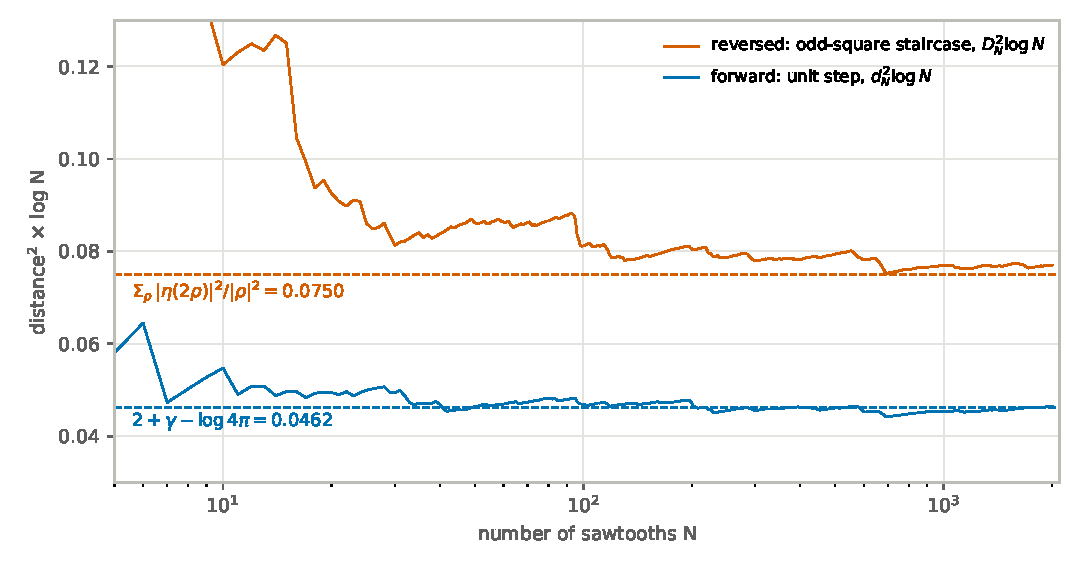
\includegraphics[width=0.92\textwidth]{fig5_staircases.pdf}
\caption{$D_N^2\log N$ for the odd-square staircase and $d_N^2\log N$ for the unit step, $5\le N\le2000$, computed from exact integrals, with the constants $C_{\mathrm{rev}}$ and $C_{\mathrm{fwd}}$ of the zeros (dashed).}\label{fig:staircases}
\end{figure}

\section{Prime clocks}\label{sec:clocks}

The clock of a prime $p$ is $t\mapsto p^{it}$; at height $t$ it reads $t\log p/2\pi$ turns. At a whole turn the clock is aligned, $p^{it}=1$; at a half turn it is reversed, $p^{it}=-1$. At $t=0$ every clock is aligned and the Euler product $\prod_p(1-p^{-s})^{-1}$ has its pole at $s=1$; turning every clock by half a turn, $p^{-s}\mapsto-p^{-s}$, gives the reversed pattern of \cref{sec:reverse}. The pitch in doublings of the wave of a zero (\cref{sec:tower}) is the reading of the clock of $2$ at its height.

\begin{proof}[Proof of \cref{mt:clocks}]
The first statement is Landau's formula \cite{Landau12}; Gonek \cite{Gonek} gives a version uniform in $x$. When $\rho=\frac12+i\gamma$, $x^\rho=\sqrt x\,\e^{i\gamma\log x}$, and taking real parts gives the mean of $\cos(\gamma\log x)$. For the clock of $p$, $\frac1{N(T)}\sum\e^{2\pi ik\gamma\log p/2\pi}=\frac1{N(T)}\sum p^{ik\gamma}=\frac{p^{-k/2}}{N(T)}\sum(p^k)^\rho$, and $\Lambda(p^k)=\log p$.
\end{proof}

With these Fourier coefficients, the density of the readings of the clock of $p$ over the zeros up to height $T$ is
\begin{equation}\label{eq:clockdensity}
\delta_p(\phi)=1-\frac{T\log p}{\pi N(T)}\sum_{k\ge1}p^{-k/2}\cos2\pi k\phi,
\end{equation}
with $\delta_p(0)=1-\frac{T\log p}{\pi N(T)(\sqrt p-1)}$ at the alignment and $\delta_p(\frac12)=1+\frac{T\log p}{\pi N(T)(\sqrt p+1)}$ at the reversal; this is the main term, each coefficient carrying an error $O(\log T/N(T))$.
Every coefficient is negative: each prime pulls the zeros toward the reversal of its clock, with strength $\Lambda(x)/\sqrt x$ at $x=p^k$. The zeros sit on the reversed side of every clock. For $p=2$, $T=3000$ and $N(T)=2469$, $\delta_2(0)=0.353$ and $\delta_2(\frac12)=1.111$.

\subsection{Measurements}

Over the $2469$ zeros with $0<\gamma<3000$, the mean of $\cos(\gamma\log x)$ agrees with Landau's formula to within $0.0012$ at every prime power up to $13$ (\cref{tab:landau}) and to within $0.0038$ at all $35$ prime powers up to $100$, the largest difference being at $x=81$. The density of the zeros on the clock of $2$ follows \eqref{eq:clockdensity} (\cref{tab:density}, \cref{fig:clocks}): near the alignment it is $0.68$ and $0.65$ of the average, and elsewhere about $1.1$.

\begin{table}[!htbp]\centering\small
\begin{tabular}{@{}lrrrrrrrrr@{}}\toprule
$x$ & $2$ & $3$ & $4$ & $5$ & $7$ & $8$ & $9$ & $11$ & $13$\\\midrule
measured & $-.0946$ & $-.1225$ & $-.0668$ & $-.1386$ & $-.1411$ & $-.0468$ & $-.0697$ & $-.1387$ & $-.1370$\\
Landau & $-.0948$ & $-.1227$ & $-.0670$ & $-.1392$ & $-.1422$ & $-.0474$ & $-.0708$ & $-.1398$ & $-.1376$\\\bottomrule
\end{tabular}
\caption{Mean of $\cos(\gamma\log x)$ over the $2469$ zeros below height $3000$, and $-\frac T{2\pi N(T)}\Lambda(x)/\sqrt x$.}\label{tab:landau}
\end{table}

\begin{table}[!htbp]\centering\small
\setlength{\tabcolsep}{4.5pt}
\begin{tabular}{@{}lrrrrrrrrrr@{}}\toprule
reading mod $1$ & $0$--$.1$ & $.1$--$.2$ & $.2$--$.3$ & $.3$--$.4$ & $.4$--$.5$ & $.5$--$.6$ & $.6$--$.7$ & $.7$--$.8$ & $.8$--$.9$ & $.9$--$1$\\\midrule
measured & $0.680$ & $0.996$ & $1.118$ & $1.065$ & $1.126$ & $1.110$ & $1.114$ & $1.077$ & $1.061$ & $0.652$\\
by \eqref{eq:clockdensity} & $0.671$ & $1.026$ & $1.088$ & $1.105$ & $1.110$ & $1.110$ & $1.105$ & $1.088$ & $1.026$ & $0.671$\\\bottomrule
\end{tabular}
\caption{Density of the zeros below height $3000$ on the clock of $2$, per tenth of a turn (average $1$).}\label{tab:density}
\end{table}

\begin{figure}[!htbp]\centering
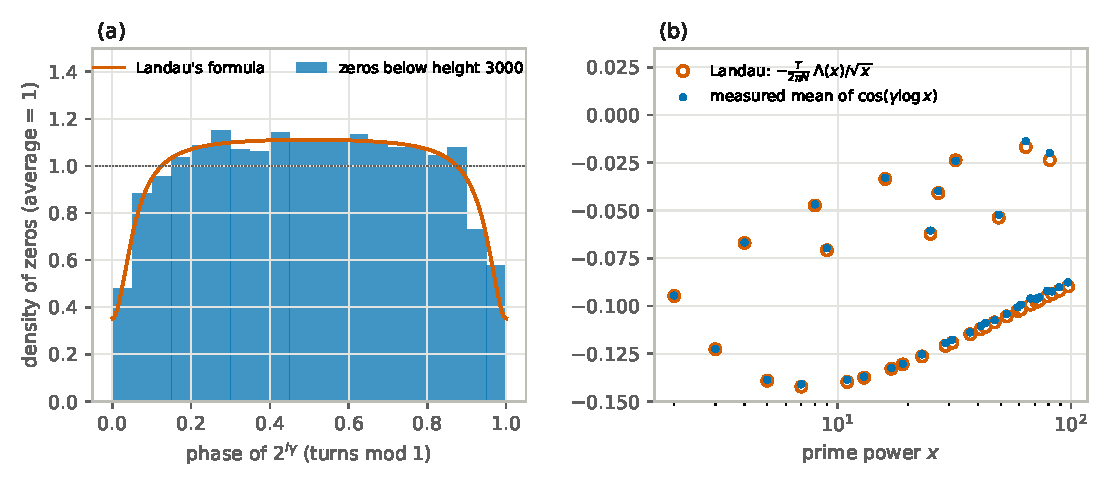
\includegraphics[width=0.95\textwidth]{fig6_prime_clocks.pdf}
\caption{(a) Density of the $2469$ zeros below height $3000$ on the clock of $2$, in twentieths of a turn, and the density \eqref{eq:clockdensity}. (b) Mean of $\cos(\gamma\log x)$ over the same zeros at the $35$ prime powers $x\le100$, and Landau's formula.}\label{fig:clocks}
\end{figure}

\paragraph{The clock of 2 in the triad charge.} Since $\chi_{-3}(2)=-1$, the Euler factor of $L(s,\chi_{-3})$ at $2$ is $(1+2^{-s})^{-1}$, whose modulus at $s=\frac12+i\gamma$ is $|1+2^{-1/2}2^{-i\gamma}|^{-1}$: $3.414$ at a half turn of the clock of $2$ and $0.586$ at a whole turn. The wave amplitudes of the triad charge $a(x)$ in \eqref{eq:amps} carry $|L(\rho,\chi_{-3})|$, and over the zeros below height $3000$ the mean of $|L(\rho,\chi_{-3})|$ is $4.24$ for the $274$ zeros within $0.05$ turn of a half turn and $0.98$ for the $130$ zeros within $0.05$ turn of a whole turn; divided by the factor at $2$, the two means are $1.38$ and $1.66$. The sixth zero, whose wave is nearly silent in the triad charge (\cref{tab:waves}), reads $4.1464$ turns, $0.15$ turn past a whole turn.

\subsection{The tenth zero}

The tenth zero $\gamma_{10}=49.7738$ reads $5.4909$ turns on the clock of $2$, within $0.009$ of $5\frac12$, which in base two is $101.1$; there $2^{i\gamma_{10}}=-0.9984+0.0569i$, and the clock is reversed. The reversed reading of \cref{mt:revNB}(iii) weights the zero by
\[
|\eta(1+2i\gamma)|^2=|1-2^{-2i\gamma}|^2\,|\zeta(1+2i\gamma)|^2,\qquad|1-2^{-2i\gamma}|=2|\sin(\gamma\log2)|,
\]
and at twice the height the clock of $2$ reads $10.9819$ turns, within $0.018$ of $11$, which in base two is $1011$: doubling the height moves the binary point one place, the half turn becomes a whole number of turns, and the factor $1-2^{1-2s}$ of $\eta(2s)$ closes. For $\gamma_{10}$, $|1-2^{-2i\gamma}|^2=0.0129$, $|\zeta(1+2i\gamma)|^2=2.04$, and the weight is $0.0264$, against a mean of $1.52$ over the $2469$ zeros.

The factor $|1-2^{-2i\gamma}|^2$ vanishes whenever the clock of $2$ reads a half or a whole turn. Of the $2469$ zeros below height $3000$, $71$ have weight below $0.05$: $49$ lie within $0.1$ turn of a half turn and $22$ within $0.1$ turn of a whole turn, more of them near the reversal, where the density \eqref{eq:clockdensity} is higher. The first seven are, as (rank, $\gamma$, reading mod $1$, weight), $(10,\,49.774,\,0.491,\,0.0264)$, $(124,\,276.452,\,0.498,\,0.0029)$, $(163,\,339.858,\,0.492,\,0.0263)$, $(172,\,353.489,\,0.996,\,0.0111)$, $(269,\,498.581,\,0.002,\,0.0016)$, $(311,\,557.565,\,0.509,\,0.0451)$ and $(327,\,580.137,\,0.999,\,0.0004)$.

\begin{remark}[rank and value]
The silence of the tenth zero in the reversed reading is a property of its value, the height $\gamma_{10}$ read on the clock of the prime $2$, and not of its rank: the same clock silences $70$ further zeros below height $3000$. That prime is $2$, written $10$ in base two.
\end{remark}

\section{Methods of computation}\label{sec:methods}

\paragraph{Counts to $10^{10}$.} The exact segmented sieve of \cite{S10} gives $\mu(n)$, $\lambda(n)$ and $\Lambda(n)$ to $10^{10}$ and records $\pi$, $M$, $L$, $\theta$, $\psi$, their restrictions to the classes $1$ and $5\bmod6$, and $\pi-\li$ in extended precision at $675{,}247$ checkpoints; it gives $\pi(10^{10})=455{,}052{,}511$, $M(10^{10})=-33{,}722$ and $L(10^{10})=-116{,}026$. The grid $u=12+0.001j$ is interpolated linearly between checkpoints; $J$ is formed from $\pi$ and a table of $\pi(y)$ for $y\le10^5$.

\paragraph{The tower.} A second segmented sieve to $10^{10}$ computes for every $n$ the values $\mu(n)$, $(\mu*\chi_{-3})(n)$ and $(\mu*\chi_{-4})(n)$ in integers and $(\mu*\chi_9)(n)$ and $(\mu*\chi_9\chi_{-3})(n)$ in $\Z[\omega]$, stored as integer pairs $(a_1,a_2)$ for $a_1+a_2\omega$ with $\omega^2=-1-\omega$, from the values at prime powers in \cref{mt:carriers}. Each $n$ is divided exactly by the primes up to $10^5$, and the cofactor left after these divisions is $1$ or a prime. All partial sums are exact and are recorded at $123{,}450$ checkpoints, which contain the grid, the points $x/3$ and the values $\lfloor10^{10}/r\rfloor$, $r\le10^5$. The leaves $M(10^{10}/r)$ come from these checkpoints for $r\le10^5$ and from a table of $M(v)$, $v\le10^5$, for $r>10^5$, and give every class of the tower at every level exactly.

\paragraph{Spectra and energies.} Mean over the grid removed, Hann window, direct evaluation of the Fourier sum at each pitch, as in \cite{S10}.

\paragraph{Zeros and special values.} The $2469$ zeros with $0<\gamma<3000$ are those of \cite{S10}, all on the critical line \cite{PT}. The functions $\zeta(s)$, $\zeta'(s)$ and $\zeta(s,a)$ are evaluated by Euler--Maclaurin summation, $L(s,\chi_{-3})=3^{-s}(\zeta(s,\frac13)-\zeta(s,\frac23))$ and $L(s,\chi_{-4})=4^{-s}(\zeta(s,\frac14)-\zeta(s,\frac34))$. The squares part is evaluated by \eqref{eq:Pinv} as $\log|E(s)|=-\sum_{2\le k\le K}\mu(k)k^{-1}\log|\zeta(ks)|$, with $K=24$ at the random points and $K=79$ for \cref{tab:halforder}.

\paragraph{Squared pair.} $Q_\zeta$ on the grid $\sigma=0.52,0.53,\dots,1.10$, $t=2+0.05j$ for \cref{fig:reach}(a); the reach by $14$ bisection steps in $\sigma$, with the minimum over $13$ equally spaced heights in $[\gamma-0.3,\gamma+0.3]$.

\paragraph{Value distribution.} $\zeta(\sigma+it)$ at $6000$ uniform random heights in $[5000,6000]$; the model as described in \cref{sec:phases}; the extremes on the grid $t=10+0.02j$.

\paragraph{Reversal.} An exact sieve of $\lambda$ to $10^8$ gives $\ell(K)$ in double precision; \eqref{eq:revrebuild} is checked by direct summation of $L$.

\paragraph{Sawtooth integrals.} As in \cref{sec:revNB}; linear algebra in double precision by Cholesky factorisation. For the recomputation and \cref{tab:exact}, $\langle f,\varsigma_k\rangle=\sum_{n\text{ odd}}\bigl(\Phi_k((n+1)^2)-\Phi_k(n^2)\bigr)$ with $\Phi_k(y)=\int_1^y\fr{u/k}u^{-2}\dd u=\bigl(\log y-H_{\lfloor y/k\rfloor}\bigr)/k+\lfloor y/k\rfloor/y$, where $H_m$ is the harmonic number. The sum runs over $n<2\cdot10^5$, and the tail is evaluated with the mean $\frac12$ of $\fr{u/k}$.

\paragraph{The identity at a zero.} The values of \cref{tab:atzero} are computed with $30$ significant digits by the mpmath library \cite{mpmath}.

\paragraph{Gaps and classes.} A sieve of the primes to $10^8$; the window law is checked directly for $p\le19$.

\section{Concluding remarks}\label{sec:concl}

\paragraph{The triad tower.} The rebuild law splits by the residue of the divisor into the self-similar tower of \cref{mt:tower}: its zero classes repeat the whole law one level down, its unit classes are the character sums $G_\chi$, carried only by the primes that the characters do not fix (\cref{mt:carriers}), and its leaves are the values $M(x/r)$, whose energy is subpolynomially above $x$ exactly when RH holds. At every zero of $\zeta$ the triad of Dirichlet series is $(0,a,-a)$ with $a=\frac12L(\rho,\chi_{-3})$ (\cref{mt:zero}), and this fixes every wave of the tower: at $10^{10}$ the class values agree exactly with the leaves, and the twelve leading wave amplitudes of $M$, $a$ and $b$ and their energies agree with the zeros to within $0.0003$ and $1\%$.

\paragraph{The squares.} Each prime square opens the next wheel (\cref{mt:gaps}): with $25$ and $49$ inserted, the primes to $61$ are the wheels of $6$ and $30$, and the classes $6k\pm1$ stand $9:9$. All squares fall in the class $6k+1$, and the logarithm of the Euler product counts each of them with weight $\frac12$ (\cref{mt:wheel}). At that weight the lean of $\pi$ against $\li$ vanishes, with fitted weight $0.4994$, and the lean of the classes $6k\pm1$ drops from $1.157$ to $0.031$, with fitted weight $0.514$; the lean of $L$ sits in its square multiples, and without them $L$ becomes $M$, which is centred. The waves are unchanged.

\paragraph{The horizon.} The squares part $E$ of $\zeta$ is analytic, zero-free and satisfies the squared-pair inequality all the way down to the square-root horizon $\sigma=\frac12$, where it has a half-order pole; the prime factor $F=\zeta/E$ carries every zero of $\zeta$ in $\sigma>\frac12$ and has at $s=\frac12$ the matching half-order zero, which is the square lean $-\frac12\li(\sqrt x)$ of the prime count (\cref{mt:horizon}, \cref{rem:halforder}). The phases $t\log p$ are jointly equidistributed on every finite torus, and in the model with independent phases the prime term has the squares series as variance and converges almost surely exactly beyond the horizon (\cref{mt:phases}); for each fixed $\sigma>\frac12$ the zeros with $\beta>\sigma$ form a proportion $O(1/\log T)$ of those up to height $T$; and the values of $\zeta$ at heights $5000$ to $6000$ follow the independent-phase law.

\paragraph{The axiom.} Harmonic independence is the absence of an integer relation (\cref{ax:harmonic}). By unique factorisation the frequencies $\log p$ of the prime waves admit none, which is a theorem (\cref{sec:axiom}); the waves are related only through the Euler product that constructs $\zeta$, and a zero off the critical line would be a relation without a mechanism.

\paragraph{The reversed pattern.} Reversing every prime turns $\zeta(s)$ into $\zeta(2s)/\zeta(s)$ and every zero into a pole; forward times reversed is $\zeta(2s)$; and the Liouville-weighted sawtooths rebuild the square staircase $\lfloor\sqrt x\rfloor$ exactly (\cref{mt:reverse}). The forward pattern has its single pole at its centre $s=1$. The reversed pattern has its centre pole at $s=\frac12$, which gives $L(x)$ its lean $\sqrt x/\zeta(\frac12)$, and its other poles at the zeros of $\zeta$. In this form the Riemann Hypothesis is the statement that every pole of the reversed pattern lies on the vertical line through its centre. The results bear on this statement from four sides. The squares part is positive and zero-free down to that line (\cref{mt:horizon}). In the independent-phase model of the prime factor, which carries the poles, the prime term converges almost surely beyond the line with the squares series as variance, and for each fixed $\sigma>\frac12$ the poles with $\beta>\sigma$ form a proportion $O(1/\log T)$ of those up to height $T$ (\cref{mt:phases}). The odd-square staircase, rebuilt exactly by the reversed sawtooths, gives the criterion that $D_N\to0$ puts every pole on the line, and computed to $N=2000$, $D_N^2\log N$ stays within $3.3\%$ of the constant $C_{\mathrm{rev}}$ of the poles on the line over $1200\le N\le2000$ (\cref{mt:revNB}, \cref{tab:DN}). Every prime clock pulls the poles toward its reversal as Landau's formula prescribes, as verified over the $2469$ poles below height $3000$ at the $35$ prime powers up to $100$ and in the density on the clock of $2$ (\cref{mt:clocks}, \cref{tab:landau,tab:density}). At each zero the forward zero and the reversed pole cancel in the product, leaving $\zeta(2\rho)$ with residue $\zeta(2\rho)/\zeta'(\rho)$. They cancel in the same way on the line and off it, so the identity holds at every zero and does not place it (\cref{prop:atzero}). The exact weights of the staircase settle the distance over $t>1$ through the vanishing of $\eta(2s)/\zeta(s)$ at $s=1$. Over $0<t\le1$ they leave an error that does not decrease up to $N=2000$ (\cref{tab:exact}), so the criterion rests on the coefficients that attain $D_N$.

\paragraph{Outlook.} The computations extend directly: the tower beyond $10^{10}$ by the rebuild law, the reversed distance $D_N$ beyond $N=2000$ by Vasyunin's closed form, and the densities of the zeros on the clocks of the odd primes by \eqref{eq:clockdensity}.

\section{Data and sources}\label{sec:data}
\paragraph{External inputs.} All inputs are mathematical; no measured data are used.
\begin{enumerate}[label=(\roman*)]
\item All nontrivial zeros of $\zeta$ with $0<\gamma\le3\cdot10^{12}$ lie on the critical line \cite{PT}.
\item Published values used for comparison: $\pi(10^n)$ \cite{OEISpi}; $M(10^{10})=-33{,}722$ \cite{OEISM}; the least $x>1$ with $L(x)>0$, $906{,}150{,}257$ \cite{Tanaka}.
\item Classical and published theorems: the rebuild law and the counts to $10^{10}$ \cite{S10}; Littlewood's criterion and the explicit formula for $M$ \cite[Theorems 14.25(C), 14.27]{Titchmarsh}; Riemann's formula for $J$ \cite{Riemann,vonMangoldt}; the prime number theorem and the explicit formula for $\psi(x,\chi)$ \cite[Ch.~18, 19]{Davenport}; the Hurwitz zeta function, $\sum_{d\mid n}\lambda(d)$ and $\sum\mu(n)/n=0$ \cite{Apostol}; Kronecker's theorem and Weyl's criterion \cite{HardyWright,Weyl}; the variance criterion and the three-series theorem \cite{KhintchineKolmogoroff,Durrett}; the mean square of $\zeta$ \cite[Theorem 7.2]{Titchmarsh} and its second term \cite{Matsumoto}; the density theorems of Bohr and Landau and of Selberg \cite{BohrLandau,Selberg46}, \cite[Theorems 9.15(A), 9.19(C)]{Titchmarsh}; the value distribution \cite{BohrJessen1,BohrJessen2}; Mertens' inequality \cite{Mertens}, \cite[\S3.3, (3.3.1)]{Titchmarsh}; Chebyshev's bias \cite{RubinsteinSarnak}; the sign changes of $\pi-\li$ \cite{Littlewood14}; Pólya's question \cite{Polya}; the criterion of Nyman, Beurling and Báez-Duarte \cite{Nyman,Beurling,BaezDuarte}; Vasyunin's closed form \cite{Vasyunin}; Burnol's bound \cite{Burnol}; the asymptotic of Bettin, Conrey and Farmer \cite{BCF}; Landau's formula \cite{Landau12,Gonek}.
\end{enumerate}
\paragraph{Computed quantities.} Every other number in the paper is computed from formulas stated in the text by the methods of \cref{sec:methods}: the tower and its waves and energies, the gaps and class counts, the leans and the fitted weights, the half-order limits and the reach of the squared pair, the value distribution and its extremes, the Liouville sums, the Gram matrices and the distances $D_N$ and $d_N$, the error of the exact weights cut at $N$, the identity at the first zeros, the constants $C_{\mathrm{fwd}}$ and $C_{\mathrm{rev}}$, and the readings and densities of the zeros on the prime clocks.

\begin{thebibliography}{99}\small
\bibitem{Apostol} T.~M.~Apostol, \emph{Introduction to Analytic Number Theory}, Undergraduate Texts in Mathematics, Springer, New York, 1976.
\bibitem{BaezDuarte} L.~B\'aez-Duarte, A strengthening of the Nyman--Beurling criterion for the Riemann hypothesis, \emph{Atti Accad. Naz. Lincei Rend. Lincei Mat. Appl.} 14 (2003) 5--11.
\bibitem{BCF} S.~Bettin, J.~B.~Conrey, D.~W.~Farmer, An optimal choice of Dirichlet polynomials for the Nyman--Beurling criterion, \emph{Proc. Steklov Inst. Math.} 280, suppl.~2 (2013) S30--S36.
\bibitem{Beurling} A.~Beurling, A closure problem related to the Riemann zeta-function, \emph{Proc. Nat. Acad. Sci. U.S.A.} 41 (1955) 312--314.
\bibitem{BohrJessen1} H.~Bohr, B.~Jessen, Über die Werteverteilung der Riemannschen Zetafunktion. Erste Mitteilung, \emph{Acta Math.} 54 (1930) 1--35.
\bibitem{BohrJessen2} H.~Bohr, B.~Jessen, Über die Werteverteilung der Riemannschen Zetafunktion. Zweite Mitteilung, \emph{Acta Math.} 58 (1932) 1--55.
\bibitem{BohrLandau} H.~Bohr, E.~Landau, Ein Satz über Dirichletsche Reihen mit Anwendung auf die $\zeta$-Funktion und die $L$-Funktionen, \emph{Rend. Circ. Mat. Palermo} 37 (1914) 269--272.
\bibitem{Burnol} J.-F.~Burnol, A lower bound in an approximation problem involving the zeros of the Riemann zeta function, \emph{Adv. Math.} 170 (2002) 56--70.
\bibitem{Davenport} H.~Davenport, \emph{Multiplicative Number Theory}, 3rd ed., revised by H.~L.~Montgomery, Graduate Texts in Mathematics 74, Springer, New York, 2000.
\bibitem{Durrett} R.~Durrett, \emph{Probability: Theory and Examples}, 5th ed., Cambridge Series in Statistical and Probabilistic Mathematics 49, Cambridge University Press, Cambridge, 2019.
\bibitem{Gonek} S.~M.~Gonek, An explicit formula of Landau and its applications to the theory of the zeta-function, in: \emph{A Tribute to Emil Grosswald: Number Theory and Related Analysis}, Contemp. Math. 143, Amer. Math. Soc., Providence, RI, 1993, 395--413.
\bibitem{HardyWright} G.~H.~Hardy, E.~M.~Wright, \emph{An Introduction to the Theory of Numbers}, 6th ed., revised by D.~R.~Heath-Brown and J.~H.~Silverman, Oxford University Press, Oxford, 2008.
\bibitem{KhintchineKolmogoroff} A.~Khintchine, A.~Kolmogoroff, Über Konvergenz von Reihen, deren Glieder durch den Zufall bestimmt werden, \emph{Mat. Sb.} 32 (1925) 668--677.
\bibitem{Landau12} E.~Landau, Über die Nullstellen der Zetafunktion, \emph{Math. Ann.} 71 (1912) 548--564.
\bibitem{Littlewood14} J.~E.~Littlewood, Sur la distribution des nombres premiers, \emph{C. R. Acad. Sci. Paris} 158 (1914) 1869--1872.
\bibitem{Matsumoto} K.~Matsumoto, The mean square of the Riemann zeta-function in the critical strip, \emph{Japan. J. Math. (N.S.)} 15 (1989) 1--13.
\bibitem{Mertens} F.~Mertens, Ueber eine Eigenschaft der Riemann'schen $\zeta$-Function, \emph{Sitzungsber. Kais. Akad. Wiss. Wien, Math.-Naturwiss. Cl.} 107 (1898) 1429--1434.
\bibitem{mpmath} The mpmath development team, \emph{mpmath: a Python library for arbitrary-precision floating-point arithmetic}, version 1.3.0, 2023, \url{https://mpmath.org/}.
\bibitem{Nyman} B.~Nyman, \emph{On Some Groups and Semigroups of Translations}, Thesis, Uppsala, 1950.
\bibitem{OEISpi} OEIS Foundation, Sequence A006880, number of primes $<10^n$, \emph{The On-Line Encyclopedia of Integer Sequences}, \url{https://oeis.org/A006880}.
\bibitem{OEISM} OEIS Foundation, Sequence A084237, $a(n)=M(10^n)$, where $M(n)$ is Mertens's function, \emph{The On-Line Encyclopedia of Integer Sequences}, \url{https://oeis.org/A084237}.
\bibitem{PT} D.~Platt, T.~Trudgian, The Riemann hypothesis is true up to $3\cdot10^{12}$, \emph{Bull. London Math. Soc.} 53 (2021) 792--797.
\bibitem{Polya} G.~Pólya, Verschiedene Bemerkungen zur Zahlentheorie, \emph{Jahresber. Deutsch. Math.-Verein.} 28 (1919) 31--40.
\bibitem{Riemann} B.~Riemann, Ueber die Anzahl der Primzahlen unter einer gegebenen Grösse, \emph{Monatsber. Königl. Preuss. Akad. Wiss. Berlin} (1859) 671--680.
\bibitem{RubinsteinSarnak} M.~Rubinstein, P.~Sarnak, Chebyshev's bias, \emph{Experiment. Math.} 3 (1994) 173--197.
\bibitem{Selberg46} A.~Selberg, Contributions to the theory of the Riemann zeta-function, \emph{Arch. Math. Naturvid.} 48 (1946) no.~5, 89--155.
\bibitem{S10} A.~Singh, The Balance of the Count: One Energy in the Prime Counts and in the Sawtooth, and the Riemann Hypothesis in Real Variables, manuscript, 2026.
\bibitem{Tanaka} M.~Tanaka, A numerical investigation on cumulative sum of the Liouville function, \emph{Tokyo J. Math.} 3 (1980) 187--189.
\bibitem{Titchmarsh} E.~C.~Titchmarsh, \emph{The Theory of the Riemann Zeta-Function}, 2nd ed., revised by D.~R.~Heath-Brown, Oxford University Press, Oxford, 1986.
\bibitem{Vasyunin} V.~I.~Vasyunin, On a biorthogonal system associated with the Riemann hypothesis, \emph{St. Petersburg Math. J.} 7 (1996) 405--419.
\bibitem{Weyl} H.~Weyl, Über die Gleichverteilung von Zahlen mod.~Eins, \emph{Math. Ann.} 77 (1916) 313--352.
\bibitem{vonMangoldt} H.~von Mangoldt, Zu Riemanns Abhandlung ``Ueber die Anzahl der Primzahlen unter einer gegebenen Grösse'', \emph{J. Reine Angew. Math.} 114 (1895) 255--305.
\end{thebibliography}
\end{document}
